\PassOptionsToPackage{unicode=true}{hyperref} % options for packages loaded elsewhere
\PassOptionsToPackage{hyphens}{url}
\PassOptionsToPackage{dvipsnames,svgnames*,x11names*}{xcolor}
%
\documentclass[11pt,french,a4paper,]{article}
\usepackage{lmodern}
\usepackage{amssymb,amsmath}
\usepackage{ifxetex,ifluatex}
\usepackage{fixltx2e} % provides \textsubscript
\ifnum 0\ifxetex 1\fi\ifluatex 1\fi=0 % if pdftex
  \usepackage[T1]{fontenc}
  \usepackage[utf8]{inputenc}
  \usepackage{textcomp} % provides euro and other symbols
\else % if luatex or xelatex
  \usepackage{unicode-math}
  \defaultfontfeatures{Ligatures=TeX,Scale=MatchLowercase}
\fi
% use upquote if available, for straight quotes in verbatim environments
\IfFileExists{upquote.sty}{\usepackage{upquote}}{}
% use microtype if available
\IfFileExists{microtype.sty}{%
\usepackage[]{microtype}
\UseMicrotypeSet[protrusion]{basicmath} % disable protrusion for tt fonts
}{}
\IfFileExists{parskip.sty}{%
\usepackage{parskip}
}{% else
\setlength{\parindent}{0pt}
\setlength{\parskip}{6pt plus 2pt minus 1pt}
}
\usepackage{xcolor}
\usepackage{hyperref}
\hypersetup{
            colorlinks=true,
            linkcolor=blue,
            filecolor=Maroon,
            citecolor=Blue,
            urlcolor=Blue,
            breaklinks=true}
\urlstyle{same}  % don't use monospace font for urls
\usepackage[margin=1in,a4paper]{geometry}
\usepackage{color}
\usepackage{fancyvrb}
\newcommand{\VerbBar}{|}
\newcommand{\VERB}{\Verb[commandchars=\\\{\}]}
\DefineVerbatimEnvironment{Highlighting}{Verbatim}{commandchars=\\\{\}}
% Add ',fontsize=\small' for more characters per line
\usepackage{framed}
\definecolor{shadecolor}{RGB}{246,246,246}
\newenvironment{Shaded}{\begin{snugshade}}{\end{snugshade}}
\newcommand{\AlertTok}[1]{\textcolor[rgb]{0.94,0.16,0.16}{#1}}
\newcommand{\AnnotationTok}[1]{\textcolor[rgb]{0.56,0.35,0.01}{\textbf{\textit{#1}}}}
\newcommand{\AttributeTok}[1]{\textcolor[rgb]{0.00,0.36,0.77}{\textbf{#1}}}
\newcommand{\BaseNTok}[1]{\textcolor[rgb]{0.00,0.81,0.14}{#1}}
\newcommand{\BuiltInTok}[1]{#1}
\newcommand{\CharTok}[1]{\textcolor[rgb]{0.31,0.60,0.02}{#1}}
\newcommand{\CommentTok}[1]{\textcolor[rgb]{0.35,0.35,0.35}{\textit{#1}}}
\newcommand{\CommentVarTok}[1]{\textcolor[rgb]{0.56,0.35,0.01}{\textbf{\textit{#1}}}}
\newcommand{\ConstantTok}[1]{\textcolor[rgb]{0.00,0.92,0.05}{#1}}
\newcommand{\ControlFlowTok}[1]{\textcolor[rgb]{0.68,0.35,0.62}{\textbf{#1}}}
\newcommand{\DataTypeTok}[1]{\textcolor[rgb]{0.13,0.29,0.53}{#1}}
\newcommand{\DecValTok}[1]{\textcolor[rgb]{0.00,0.00,0.81}{#1}}
\newcommand{\DocumentationTok}[1]{\textcolor[rgb]{0.56,0.35,0.01}{\textbf{\textit{#1}}}}
\newcommand{\ErrorTok}[1]{\textcolor[rgb]{0.64,0.00,0.00}{\textbf{#1}}}
\newcommand{\ExtensionTok}[1]{\textcolor[rgb]{0.75,0.31,0.31}{#1}}
\newcommand{\FloatTok}[1]{\textcolor[rgb]{0.00,0.00,0.81}{#1}}
\newcommand{\FunctionTok}[1]{\textcolor[rgb]{0.60,0.00,1.00}{#1}}
\newcommand{\ImportTok}[1]{#1}
\newcommand{\InformationTok}[1]{\textcolor[rgb]{0.56,0.35,0.01}{\textbf{\textit{#1}}}}
\newcommand{\KeywordTok}[1]{\textcolor[rgb]{0.68,0.35,0.62}{\textbf{#1}}}
\newcommand{\NormalTok}[1]{#1}
\newcommand{\OperatorTok}[1]{\textcolor[rgb]{0.81,0.36,0.00}{\textbf{#1}}}
\newcommand{\OtherTok}[1]{\textcolor[rgb]{0.56,0.35,0.01}{#1}}
\newcommand{\PreprocessorTok}[1]{\textcolor[rgb]{0.56,0.35,0.01}{\textit{#1}}}
\newcommand{\RegionMarkerTok}[1]{#1}
\newcommand{\SpecialCharTok}[1]{\textcolor[rgb]{0.35,0.00,0.31}{#1}}
\newcommand{\SpecialStringTok}[1]{\textcolor[rgb]{0.31,0.60,0.02}{#1}}
\newcommand{\StringTok}[1]{\textcolor[rgb]{0.31,0.60,0.02}{#1}}
\newcommand{\VariableTok}[1]{\textcolor[rgb]{0.90,0.33,0.00}{#1}}
\newcommand{\VerbatimStringTok}[1]{\textcolor[rgb]{0.30,0.62,0.00}{#1}}
\newcommand{\WarningTok}[1]{\textcolor[rgb]{0.56,0.35,0.01}{\textbf{\textit{#1}}}}
\usepackage{longtable,booktabs}
% Fix footnotes in tables (requires footnote package)
\IfFileExists{footnote.sty}{\usepackage{footnote}\makesavenoteenv{longtable}}{}
\usepackage{graphicx,grffile}
\makeatletter
\def\maxwidth{\ifdim\Gin@nat@width>\linewidth\linewidth\else\Gin@nat@width\fi}
\def\maxheight{\ifdim\Gin@nat@height>\textheight\textheight\else\Gin@nat@height\fi}
\makeatother
% Scale images if necessary, so that they will not overflow the page
% margins by default, and it is still possible to overwrite the defaults
% using explicit options in \includegraphics[width, height, ...]{}
\setkeys{Gin}{width=\maxwidth,height=\maxheight,keepaspectratio}
\setlength{\emergencystretch}{3em}  % prevent overfull lines
\providecommand{\tightlist}{%
  \setlength{\itemsep}{0pt}\setlength{\parskip}{0pt}}
\setcounter{secnumdepth}{5}
% Redefines (sub)paragraphs to behave more like sections
\ifx\paragraph\undefined\else
\let\oldparagraph\paragraph
\renewcommand{\paragraph}[1]{\oldparagraph{#1}\mbox{}}
\fi
\ifx\subparagraph\undefined\else
\let\oldsubparagraph\subparagraph
\renewcommand{\subparagraph}[1]{\oldsubparagraph{#1}\mbox{}}
\fi

% set default figure placement to htbp
\makeatletter
\def\fps@figure{htbp}
\makeatother

\usepackage{sectsty}
\usepackage{hyperref}
\usepackage{listings}

\usepackage{wrapfig}
\usepackage{float}

\sectionfont{\clearpage\LARGE\underline\boldmath}
\subsectionfont{\Large\boldmath}
\subsubsectionfont{\large}
\paragraphfont{\large}

\def\myauthor{Anonyme}

\hypersetup{
	pdftitle={MAPR},
	pdfauthor={Marcus Hamelink},
	pdfsubject={Raycasting algorithm},
	pdfkeywords={raycasting rendering}
}
\ifnum 0\ifxetex 1\fi\ifluatex 1\fi=0 % if pdftex
  \usepackage[shorthands=off,main=french]{babel}
\else
  % load polyglossia as late as possible as it *could* call bidi if RTL lang (e.g. Hebrew or Arabic)
  \usepackage{polyglossia}
  \setmainlanguage[]{french}
\fi

\date{}

\begin{document}

\begin{titlepage}
	\begin{center}
		\vspace*{1cm}

		\Huge
		\textbf{MAPR: \\ Méthode Algorithmique Pour Rendu 3D}

		\vspace{0.5cm}
		\LARGE
		Création d’un algorithme de rendu d’images en 3 dimensions 

		\vspace{1.5cm}

		\textbf{\myauthor}

		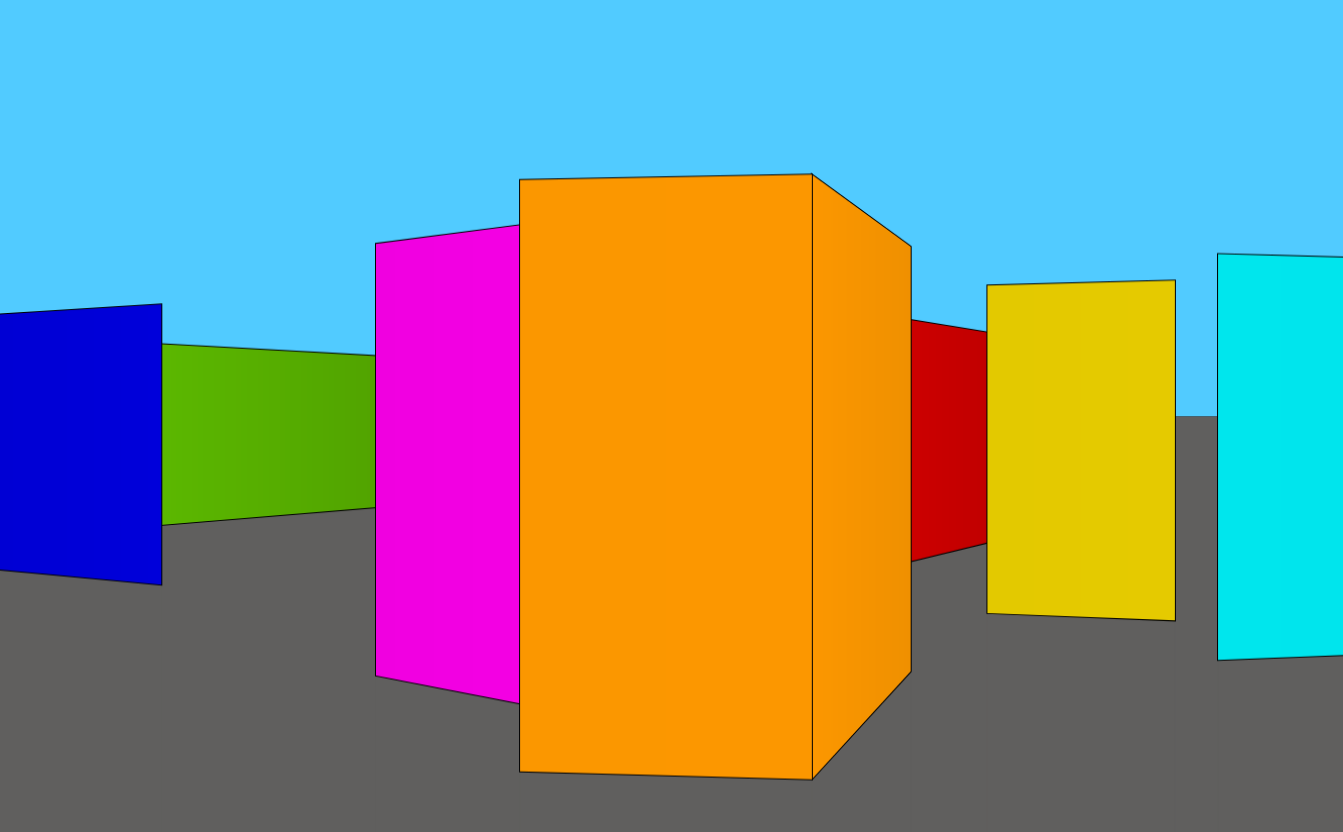
\includegraphics{../img/CoverPic/Main_Pic4.png}

		\vfill
		Un projet d'abord présenté comme travail de Maturité \\
		puis développé pour le Prix Informatique
				
		\vspace{0.8cm}
		
		\Large
		Collège de Candolle \\
		24 mars 2022
	\end{center}
\end{titlepage}



\thispagestyle{empty}

{
\hypersetup{linkcolor=}
\setcounter{tocdepth}{3}
\tableofcontents
}
\hypertarget{introduction}{%
\section{Introduction}\label{introduction}}

Après avoir appris à programmer en Python en mars 2020 au début du
confinement, je suis devenu fasciné par tout ce qui est informatique. Je
n'ai pas arrêté d'apprendre des nouvelles notions de programmation et,
durant l'été, j'ai commencé à apprendre Javascript pour coder des sites
web. J'ai été notamment intéressé par la création de jeux.

Au début de ma troisième année du collège, j'ai découvert le
\emph{Raycasting}, qui est une ``technique de calcul d'images de
synthèse 3D''\footnote{Raycasting. Wikipédia : l'encyclopédie libre
  {[}en ligne{]}. Dernière modification de la page le 22 juillet 2021 à
  22:17. {[}Consulté le 2 octobre 2021{]}. Disponible à l'adresse :
  \url{https://fr.wikipedia.org/wiki/Raycasting}}. C'est ce qui a rendu
possible les premiers jeux vidéo en 3D comme \emph{Doom} ou
\emph{Wolfenstein} 3D au début des années 1990. Fondée sur un espace en
2D et non pas sur un monde 3D, la méthode permet de simuler une
perspective en 3D sans les calculs complexes de la troisième dimension.
J'expliquerai de manière plus détaillée comment cette technique
fonctionne dans le développement.

J'ai alors commencé à apprendre comment implémenter cette méthode
moi-même en suivant des guides sur internet et c'est alors que j'ai
décidé d'en faire mon travail de Maturité. Initialement, mon plan était
de créer un moteur de jeu avec un grand nombre de fonctionnalités qui
auraient permis à quiconque de dessiner des environnements sur un plan
et de les explorer en perspective. Il y aurait également eu un accès
facile à mon code pour programmer des nouveaux jeux avec mes bases.

Peu de temps après, je me suis rendu compte que la méthode que
j'utilisais ne me plaisait pas visuellement et je voulais exploiter les
capacités des ordinateurs modernes. J'ai donc décidé de chercher à créer
ma propre technique suivant les principes du Raycasting. Les notions de
géométrie vectorielle que j'ai apprises lors de mes cours de maths en
troisième année du collège m'ont énormément aidé pour appliquer les
mathématiques dans mon code.

Après avoir rendu ce projet de Maturité, j'ai continué à travailler
dessus dans mon temps libre. Ce document présente les explications
originales avec des mentions des fonctionnalités que j'ai améliorées ou
ajoutées.

Dans ce rapport, je détaillerai d'abord comment accéder à une démo du
projet final ainsi qu'un guide de son utilisation. J'expliquerai ensuite
les principes des méthodes actuelles du Raycasting. Enfin, je décrirai
les nouvelles fonctionnalités qui composent ma méthode.

\hypertarget{informations-sur-le-projet}{%
\section{Informations sur le projet}\label{informations-sur-le-projet}}

\hypertarget{choix-du-langage}{%
\subsection{Choix du langage}\label{choix-du-langage}}

J'ai écrit le code pour ce projet avec \emph{VSCode} qui est un éditeur
de texte pour programmer. Il peut être exécuté en ouvrant le fichier
\emph{index.html} avec n'importe navigateur internet \emph{(Chrome,
Firefox, Safari, etc.)}.

J'ai choisi de développer mon projet comme un site web qui serait alors
accessible un navigateur internet, y compris ceux trouvés sur un
smartphone. Ce choix a été motivé par l'envie de pouvoir facilement
partager ma création avec des amis. Un site web moderne est généralement
developpé en combinant 3 langages de programmation différents.

\begin{itemize}
\item
  \textbf{HTML} (HyperText Markup Language) permettant de décrire le
  contenu statique (texte formaté, images, etc.) inclus sur la page.
\item
  \textbf{CSS} (Cascading Style Sheets) pour personnaliser l'apparence
  du contenu défini dans la partie HTML, en tenant compte de l'appareil
  sur lequel le site est affiché Pour se rendre compte de l'importance
  du \emph{CSS}, voici une comparaison de l'interface pour ordinateur
  avec et sans style appliqué :

  \begin{longtable}[]{@{}cc@{}}
  \toprule
  \endhead
  \begin{minipage}[t]{0.47\columnwidth}\centering
  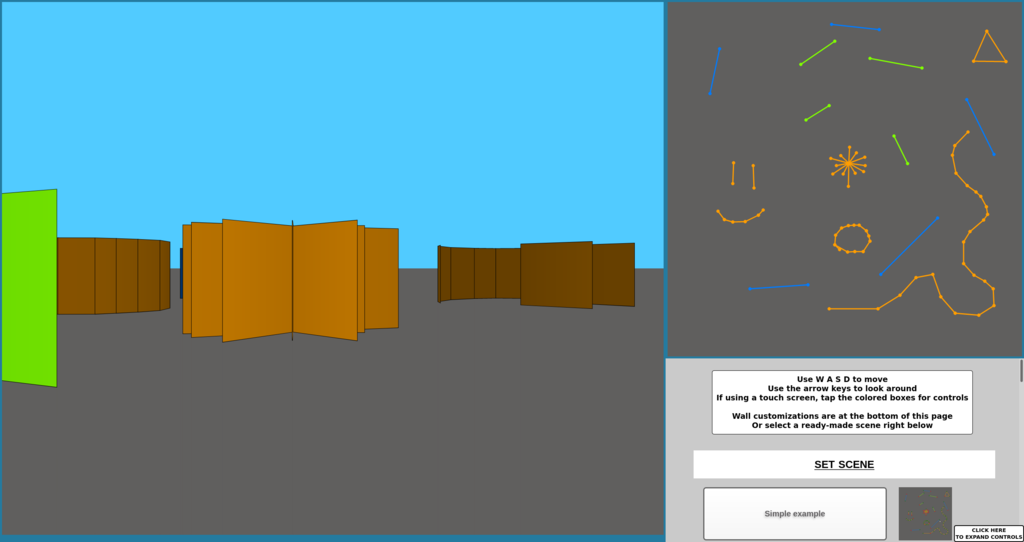
\includegraphics[width=\textwidth,height=1.66667in]{../img/PageScreenshot/resizeFullCSS.png}\strut
  \end{minipage} & \begin{minipage}[t]{0.47\columnwidth}\centering
  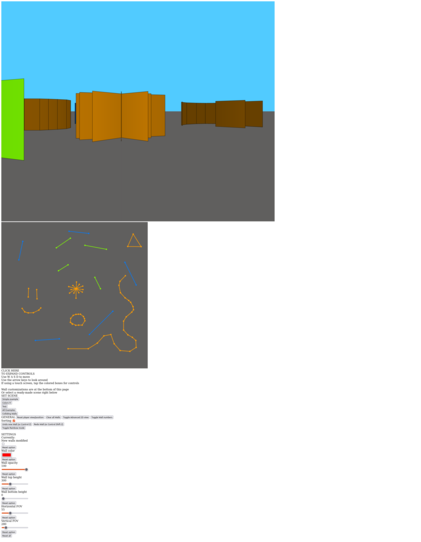
\includegraphics[width=\textwidth,height=1.66667in]{../img/PageScreenshot/resizeNoCSS.png}\strut
  \end{minipage}\tabularnewline
  \begin{minipage}[t]{0.47\columnwidth}\centering
  Page du projet avec style appliqué\footnotemark{}\strut
  \end{minipage}
  \footnotetext{Démonstration du projet hébergé sur
    \url{https://mapr.me/}} &
  \begin{minipage}[t]{0.47\columnwidth}\centering
  Page du projet sans style\strut
  \end{minipage}\tabularnewline
  \bottomrule
  \end{longtable}
\item
  \textbf{Javascript} Un langage de programmation multi-usage qui donne
  la possibilité au programmeur de manipuler la page web de manière
  dynamique en modifiant les éléments affichés.
\end{itemize}

Afin de faciliter le développement dans ces trois langages différents,
j'ai choisi d'utiliser l'éditeur de texte VSCode, un choix très commun
pour ce type de projet.

Ce projet a été réalisé sans aucune dépendance, c'est-à-dire que je n'ai
recouru à aucune librairie téléchargée pour m'aider.

\hypertarget{instructions-pour-lutilisation-de-lapplication}{%
\subsection{Instructions pour l'utilisation de
l'application}\label{instructions-pour-lutilisation-de-lapplication}}

La page de mon projet est divisée en trois parties :

\begin{itemize}
\tightlist
\item
  La projection 3D de l'environnement depuis la perspective en première
  personne du joueur
\item
  Le plan à vue d'oiseau du niveau interactif
\item
  La section paramètres défilable permettant à l'utilisateur de
  personaliser l'apparence de la projection
\end{itemize}

Sur un appareil avec un clavier, le joueur peut être déplacé avec les
touches W, A, S et D. Pour orienter le regard du joueur de gauche à
droite ou de haut en bas, les touches fléchées sont utilisées. Sur un
écran tactile où il n'y a pas de clavier, des touches virtuelles sont
dessinées sur la projection 3D.

Des obstacles peuvent être dessinés sur le plan à vue d'oiseau en
cliquant et en faisant glisser la souris dessus (ou le doigt sur les
écrans tactiles). En maintenant la touche \emph{Majuscule} lorsque vous
dessinez un obstacle, le curseur va se coller automatiquement à
l'extrémité de l'obstacle le plus proche. Cette fonctionnalité existe
aussi sur les écrans tactiles, mais elle se fait automatiquement lorsque
l'extrémité est déjà placée.

La section paramètres contient tout ce qu'il faut pour modifier
l'apparence des obstacles (couleur, position en hauteur, etc.).
Néanmoins, une sélection rapide de différents plans déjà créés sont
disponibles au début de la section. Ces plans ont été dessinés pour
montrer les capacités de mon programme. Ils se trouvent également
plusieurs options qui facilitent l'exposition des fonctionnalités du
projet et qui m'ont aidé à régler certains problèmes d'affichage. Si
cette section est trop petite sur la page, un bouton au coin en bas à
droite permet de l'élargir.

\hypertarget{description-de-la-technique-de-raycasting}{%
\section{Description de la technique de
Raycasting}\label{description-de-la-technique-de-raycasting}}

J'ai d'abord découvert le Raycasting grâce à une vidéo par Daniel
Shiffman, un créateur sur YouTube qui tient la chaîne \emph{The Coding
Train}, où dans une de ses séries, \emph{Coding challenge}, il réalise
des petits projets dans le but d'éduquer ses auditeurs. Sa vidéo sur le
Raycasting\footnote{SHIFFMAN Daniel, 2019 Coding Challenge \#146 :
  Rendering Raycasting {[}enregistrement vidéo{]}. YouTube {[}en
  ligne{]}. Disponible à l'adresse : \url{https://youtu.be/vYgIKn7iDH8}.}
a été pour moi une bonne introduction au sujet. J'ai passé de nombreuses
heures à comprendre les principes afin de pouvoir les appliquer dans mes
propres projets. J'ai décidé d'en faire mon travail de Maturité, car
j'étais curieux de savoir comment je pouvais créer mes propres jeux
avec.

La méthode la plus courante et celle que j'ai codée en premier est la
suivante : On part d'un plan en 2 dimensions où le joueur est représenté
par un point ainsi que deux segments indiquant l'étendue de son champ de
vision (indiqueé ci-dessous en orange). Autour de lui sont placés des
traits qui représentent des obstacles (en vert). Le joueur peut se
déplacer et de s'orienter librement sur le plan.

\begin{longtable}[]{@{}c@{}}
\toprule
\endhead
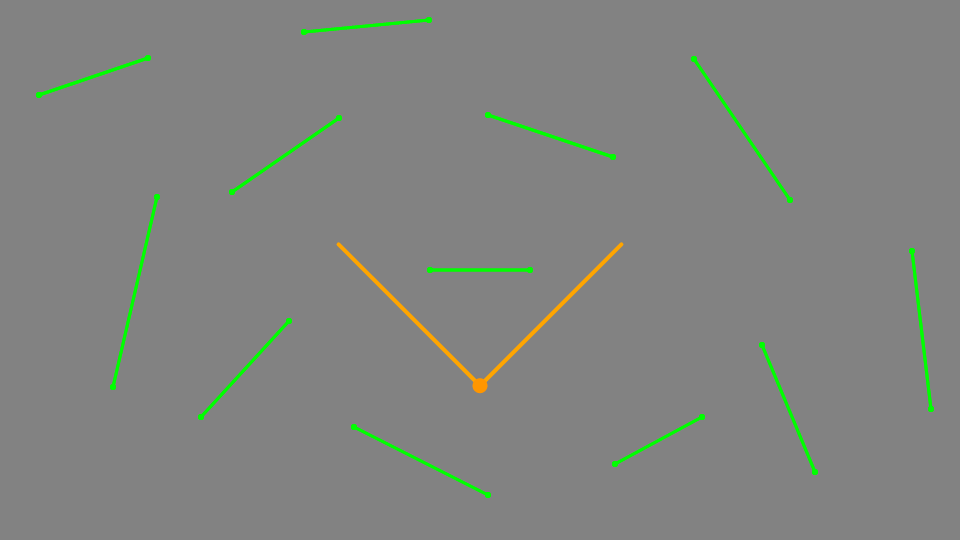
\includegraphics[width=0.8\textwidth,height=\textheight]{../img/Basic_level_player.png}\tabularnewline
Plan 2D du joueur entouré d'obstacles\tabularnewline
\bottomrule
\end{longtable}

Dans mon programme, tous les obstacles ainsi que le joueur sont
représentés dans mon programme sous forme ``d'objets Javascript''.
C'est-à-dire que chacun d'eux possède des propriétés qui leur
correspondent individuellement. Telles que les coordonnées x, y sur le
plan, l'orientation, la couleur, etc.

Ensuite, on génère des rayons provenant du joueur entre les extrémités
de son champ de vision. Lorsque les rayons intersectent avec un
obstacle, on calcule le point d'intersection où se joignent les deux
segments\footnote{Le développement de la formule mathématique de
  l'intersection se trouve en Annexe a)}.

Le plan 2D n'est qu'une représentation des calculs réalisés pour le
rendu 3D. Ainsi, on peut se balader sur le plan comme si on se trouvait
à la place du point et on percevait tous les obstacles de nos propres
yeux sur le sol.

\begin{longtable}[]{@{}cc@{}}
\toprule
\endhead
\begin{minipage}[t]{0.47\columnwidth}\centering
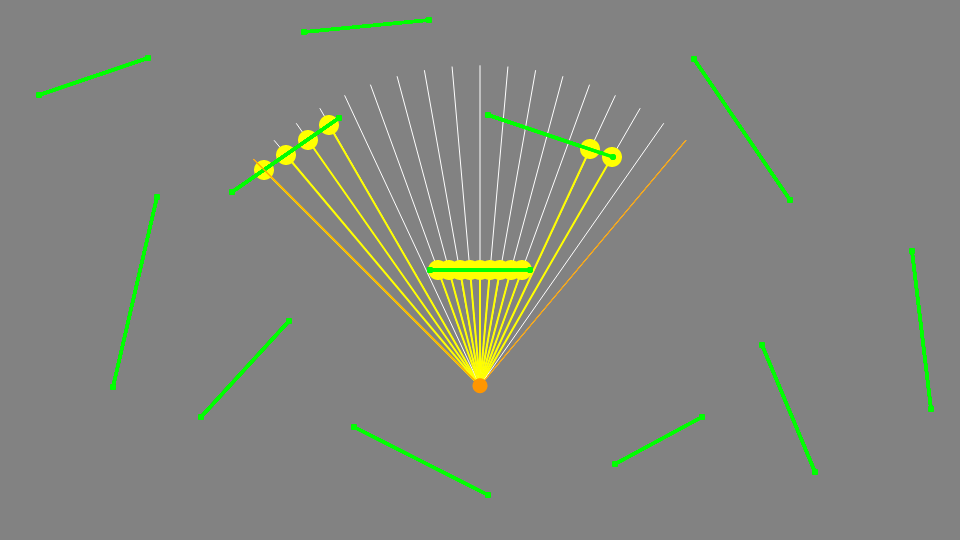
\includegraphics{../img/IntersectionComparison/rays_intersections.png}\strut
\end{minipage} & \begin{minipage}[t]{0.47\columnwidth}\centering
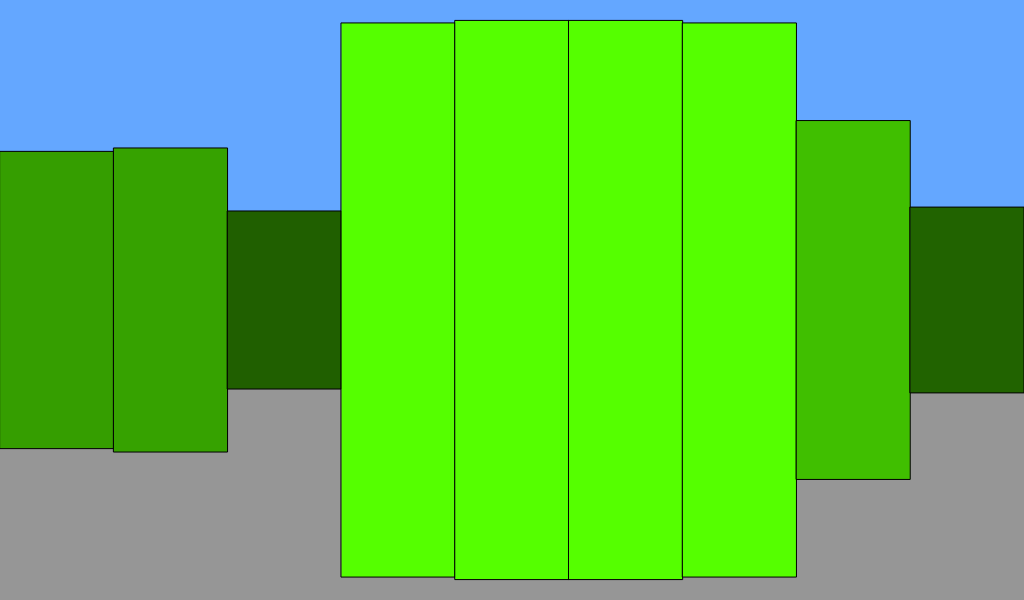
\includegraphics{../img/IntersectionComparison/3d_simple_raycast.png}\strut
\end{minipage}\tabularnewline
\begin{minipage}[t]{0.47\columnwidth}\centering
Plan 2D avec 18 points d'intersection calculés\strut
\end{minipage} & \begin{minipage}[t]{0.47\columnwidth}\centering
Perspective 3D calculée à partir du plan 2D\strut
\end{minipage}\tabularnewline
\begin{minipage}[t]{0.47\columnwidth}\centering
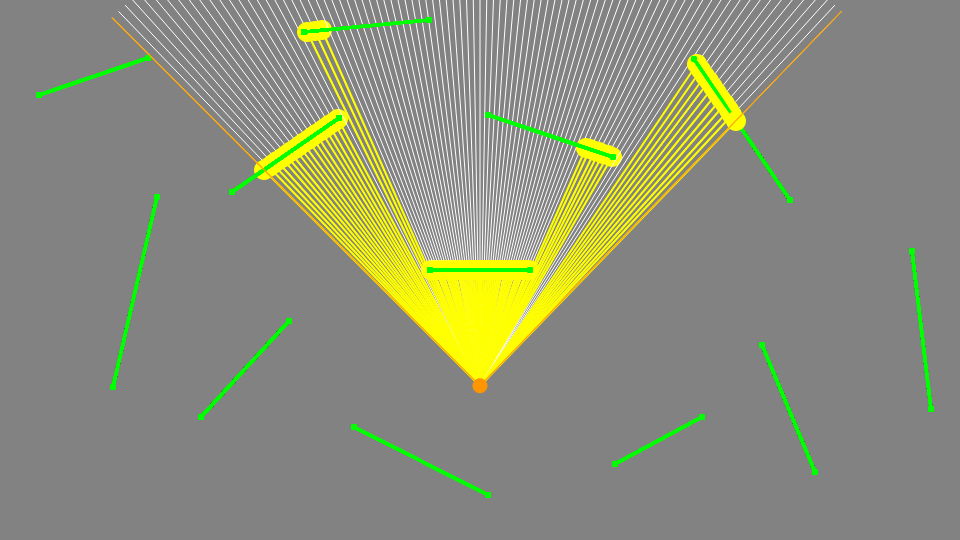
\includegraphics{../img/IntersectionComparison/rays_intersections_more.png}\strut
\end{minipage} & \begin{minipage}[t]{0.47\columnwidth}\centering
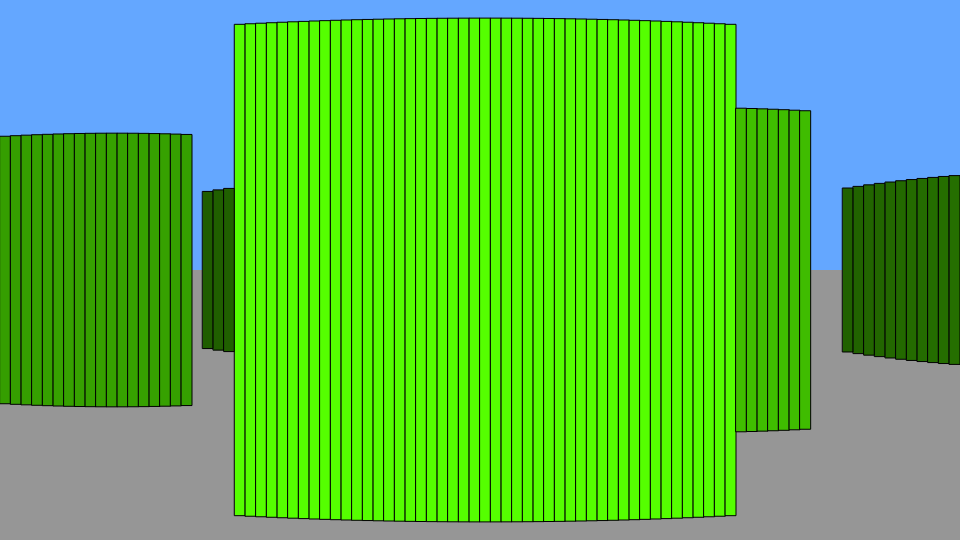
\includegraphics{../img/IntersectionComparison/3d_simple_raycast_more.png}\strut
\end{minipage}\tabularnewline
\begin{minipage}[t]{0.47\columnwidth}\centering
Plan 2D avec 90 points d'intersections\strut
\end{minipage} & \begin{minipage}[t]{0.47\columnwidth}\centering
Même perspective avec plus de détails\strut
\end{minipage}\tabularnewline
\bottomrule
\end{longtable}

Sur les images ci-dessus, on peut observer une représentation (à gauche)
du plan 2D et (à droite) la perspective 3D.

L'écran de la perspective 3D est divisé horizontalement par le nombre de
rayons générés. Ainsi, pour chacun de ces rayons, on lui associe une
partie de cet écran 3D et on utilise la distance entre le joueur et
l'intersection avec un obstacle pour dessiner un rectangle à hauteur
proportionnelle à la distance. C'est-à-dire, si la distance est plus
grande, l'intersection se trouve plus loin du joueur donc la hauteur du
rectangle sera plus petite et vice versa si la distance est plus petite.
Ceci permet de simuler la perspective que l'on aperçoit de nos propres
yeux.

Les images ci-dessus sont une démonstration de ce concept avec d'un côté
ce qui se passe sur le plan 2D et de l'autre ce qu'on peut apercevoir
après les calculs d'images. Pour calculer la hauteur du rectangle, il
existe une autre manière que j'applique dans ma nouvelle méthode pour
ces calculs d'images 3D.

Il existe également d'autres méthodes pour coder un moteur de rendu avec
le Raycasting, comme à partir d'une grille pour présenter les obstacles
comme des cubes\footnote{Il existe un guide complet pour réaliser cette
  méthode, Raycasting, Lode Vandevenne, 2004-2020, Disponible à
  l'adresse : \url{https://lodev.org/cgtutor/raycasting.html}}, le
principe basique est le même. C'est à partir de ce principe expliqué
précédemment que j'ai créé une nouvelle méthode qui me plaisait mieux.

\hypertarget{les-principes-de-ma-nouvelle-muxe9thode}{%
\section{Les principes de ma nouvelle
méthode}\label{les-principes-de-ma-nouvelle-muxe9thode}}

\hypertarget{concept}{%
\subsection{Concept}\label{concept}}

Ce que je n'aimais pas avec la méthode initiale, c'était l'aspect
pixelisé du rendu 3D. Lorsque le joueur se dirige dans une autre
direction, on voit un changement dans les rectangles qui sont dessinés,
cassant cette perspective que l'on perçoit de nos propres yeux.

En revanche, plus on utilise de rayons, plus il y a de rectangles qui
sont dessinés. Seulement, une augmentation de calculs par image entraîne
rapidement un ralentissement de l'expérience de jeu et limite les
possibilités, surtout si en plus du nombre de rayons, on augmente
également le nombre d'obstacles. De plus, on a moins de liberté si on
veut, par exemple, dessiner un contour autour des obstacles (étant donné
qu'il n'y a pas d'unique forme, mais une multitude de rectangles qui ont
chacun leur propre contour).

Ainsi, je me suis dit que je pouvais utiliser des polygones pour
dessiner ces obstacles, car peu importe l'orientation des obstacles, la
perspective qui en résulte sera toujours un polygone à quatre coins. Le
problème, c'est qu'avec la méthode précédente, on ne sait pas si deux
rayons intersectent avec un même obstacle. On aurait éventuellement pu
le détecter, mais un autre problème se pose lorsque le coin d'un
obstacle se trouve entre deux rayons. Il suffit que le joueur se déplace
un tout petit peu et le coin de cet obstacle dans la perspective 3D ne
sera pas au même endroit.

\begin{longtable}[]{@{}cc@{}}
\toprule
\endhead
\begin{minipage}[t]{0.47\columnwidth}\centering
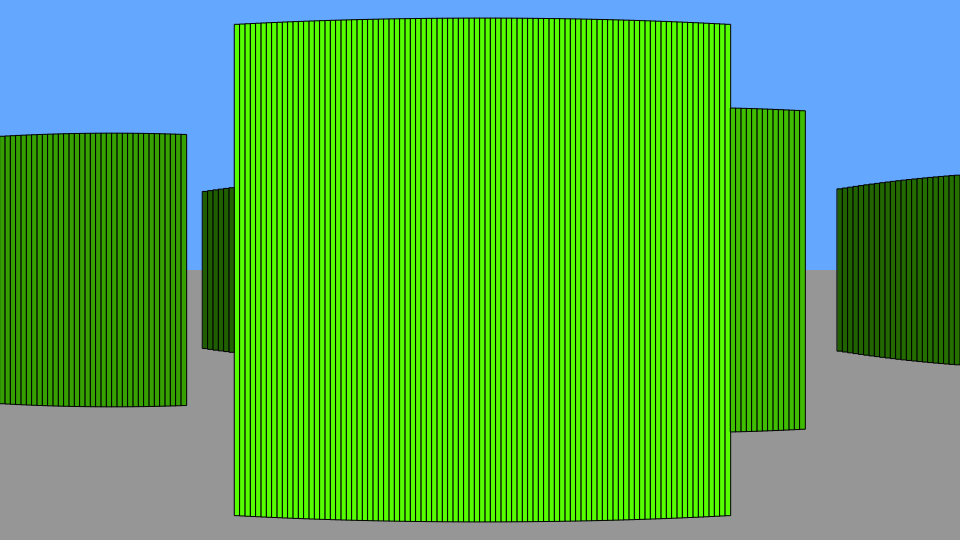
\includegraphics{../img/OldVSNew/VS_Old.png}\strut
\end{minipage} & \begin{minipage}[t]{0.47\columnwidth}\centering
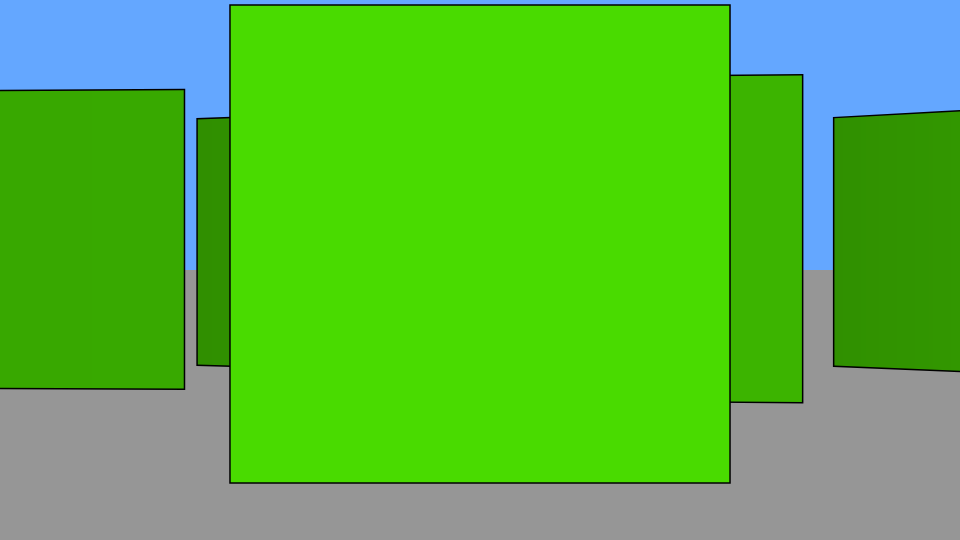
\includegraphics{../img/OldVSNew/VS_New.png}\strut
\end{minipage}\tabularnewline
\begin{minipage}[t]{0.47\columnwidth}\centering
Perspective 3D de l'ancienne méthode 180 rayons
calculés{[}\^{}oldvsnew{]}\strut
\end{minipage} & \begin{minipage}[t]{0.47\columnwidth}\centering
Perspective 3D de ma nouvelle méthode 10 rayons calculés\strut
\end{minipage}\tabularnewline
\bottomrule
\end{longtable}

Ce sont ces petits détails qui m'ont fait comprendre que si je voulais
changer de méthode, je devais supprimer cette génération de tous ces
rayons. En gardant cette idée de dessiner des polygones, on peut en
déduire une nouvelle manière de détecter les obstacles.

Dans cette section, je vais présenter les différentes fonctions
utilisées par mon programme. Ces fonctions sont exécutées sur chacun des
obstacles.

\hypertarget{duxe9tecter-les-obstacles-dans-le-champ-de-vision}{%
\subsection{Détecter les obstacles dans le champ de
vision}\label{duxe9tecter-les-obstacles-dans-le-champ-de-vision}}

Pour commencer, il faut regrouper tous les obstacles qui se situent dans
le champ de vision du joueur. La fonction \texttt{isInsideFOV()} (qui
signifie ``se trouvant à l'intérieur du champ de vision'' en anglais)
attribue d'abord deux nouvelles variables \texttt{p} et \texttt{h} qui
sont deux vecteurs qui relient respectivement la position du joueur à
chacune des extrémités de l'obstacle. (\texttt{p} qui signifie position
et qui correspond au vecteur du premier point de l'obstacle et
\texttt{h} qui signifie header, aussi dit l'entête de l'obstacle)

Ensuite, on effectue la vérification par l'utilisation répétée de
\texttt{isClockwiseOrder()}\footnote{Voir point b) de l'Annexe pour une
  explication détaillée de cette fonction}, une fonction qui prend deux
vecteurs et qui retourne vrai si le premier est orienté dans le sens des
aiguilles d'une montre par rapport au deuxième.

Dans mon programme, si une des extrémités de l'obstacle est à la fois à
la droite du vecteur de champ de vision de gauche et aussi à la gauche
du vecteur de champ de vision de droite, alors la fonction va retourner
vrai. On vérifie ceci pour les deux extrémités. De plus, si le joueur
observe un obstacle de près et que les extrémités sortent du champ de
vision, la fonction vérifie également s'il existe une
intersection\footnote{La fonction \emph{isIntersection()} dont
  l'explication se trouve dans l'Annexe a)} entre l'obstacle et chacun
des vecteurs de champ de vision.

Cette fonction permet d'effectuer les prochains calculs seulement sur
les obstacles qui comptent.

\begin{Shaded}
\begin{Highlighting}[]
\KeywordTok{function} \AttributeTok{isInsideFOV}\NormalTok{() }\OperatorTok{\{}
\CommentTok{// Creating vector going from player to wall's first vertex}
    \KeywordTok{this}\NormalTok{.}\AttributeTok{p} \OperatorTok{=} \OperatorTok{\{}
        \StringTok{'x'}\OperatorTok{:} \KeywordTok{this}\NormalTok{.}\VariableTok{pos}\NormalTok{.}\AttributeTok{x} \OperatorTok{-} \VariableTok{player}\NormalTok{.}\VariableTok{pos}\NormalTok{.}\AttributeTok{x}\OperatorTok{,}
        \StringTok{'y'}\OperatorTok{:} \KeywordTok{this}\NormalTok{.}\VariableTok{pos}\NormalTok{.}\AttributeTok{y} \OperatorTok{-} \VariableTok{player}\NormalTok{.}\VariableTok{pos}\NormalTok{.}\AttributeTok{y}
    \OperatorTok{\};}

\CommentTok{// Creating vector going from player to wall's first vertex}
    \KeywordTok{this}\NormalTok{.}\AttributeTok{h} \OperatorTok{=} \OperatorTok{\{}
        \StringTok{'x'}\OperatorTok{:}\NormalTok{ (}\KeywordTok{this}\NormalTok{.}\VariableTok{pos}\NormalTok{.}\AttributeTok{x} \OperatorTok{+} \KeywordTok{this}\NormalTok{.}\VariableTok{dir}\NormalTok{.}\AttributeTok{x}\NormalTok{) }\OperatorTok{-} \VariableTok{player}\NormalTok{.}\VariableTok{pos}\NormalTok{.}\AttributeTok{x}\OperatorTok{,}
        \StringTok{'y'}\OperatorTok{:}\NormalTok{ (}\KeywordTok{this}\NormalTok{.}\VariableTok{pos}\NormalTok{.}\AttributeTok{y} \OperatorTok{+} \KeywordTok{this}\NormalTok{.}\VariableTok{dir}\NormalTok{.}\AttributeTok{y}\NormalTok{) }\OperatorTok{-} \VariableTok{player}\NormalTok{.}\VariableTok{pos}\NormalTok{.}\AttributeTok{y}
    \OperatorTok{\};}

    \KeywordTok{this}\NormalTok{.}\VariableTok{p}\NormalTok{.}\AttributeTok{dist} \OperatorTok{=} \VariableTok{Math}\NormalTok{.}\AttributeTok{sqrt}\NormalTok{((}\KeywordTok{this}\NormalTok{.}\VariableTok{p}\NormalTok{.}\AttributeTok{x}\NormalTok{) }\OperatorTok{**} \DecValTok{2} \OperatorTok{+}\NormalTok{ (}\KeywordTok{this}\NormalTok{.}\VariableTok{p}\NormalTok{.}\AttributeTok{y}\NormalTok{) }\OperatorTok{**} \DecValTok{2}\NormalTok{)}\OperatorTok{;}
    \KeywordTok{this}\NormalTok{.}\VariableTok{h}\NormalTok{.}\AttributeTok{dist} \OperatorTok{=} \VariableTok{Math}\NormalTok{.}\AttributeTok{sqrt}\NormalTok{((}\KeywordTok{this}\NormalTok{.}\VariableTok{h}\NormalTok{.}\AttributeTok{x}\NormalTok{) }\OperatorTok{**} \DecValTok{2} \OperatorTok{+}\NormalTok{ (}\KeywordTok{this}\NormalTok{.}\VariableTok{h}\NormalTok{.}\AttributeTok{y}\NormalTok{) }\OperatorTok{**} \DecValTok{2}\NormalTok{)}\OperatorTok{;}

    \ControlFlowTok{if}\NormalTok{ ((}\AttributeTok{isIntersectionFovW}\NormalTok{(}\VariableTok{player}\NormalTok{.}\VariableTok{fov}\NormalTok{.}\AttributeTok{v1}\OperatorTok{,} \KeywordTok{this}\NormalTok{) }\OperatorTok{||}
            \AttributeTok{isIntersectionFovW}\NormalTok{(}\VariableTok{player}\NormalTok{.}\VariableTok{fov}\NormalTok{.}\AttributeTok{v2}\OperatorTok{,} \KeywordTok{this}\NormalTok{)}
\NormalTok{        ) }\OperatorTok{||}
\NormalTok{        (}\AttributeTok{isClockwiseOrder}\NormalTok{(}\VariableTok{player}\NormalTok{.}\VariableTok{fov}\NormalTok{.}\VariableTok{v1}\NormalTok{.}\AttributeTok{dir}\OperatorTok{,} \KeywordTok{this}\NormalTok{.}\AttributeTok{p}\NormalTok{) }\OperatorTok{&&}
            \OperatorTok{!}\AttributeTok{isClockwiseOrder}\NormalTok{(}\VariableTok{player}\NormalTok{.}\VariableTok{fov}\NormalTok{.}\VariableTok{v2}\NormalTok{.}\AttributeTok{dir}\OperatorTok{,} \KeywordTok{this}\NormalTok{.}\AttributeTok{p}\NormalTok{) }\OperatorTok{&&}
            \AttributeTok{isClockwiseOrder}\NormalTok{(}\VariableTok{player}\NormalTok{.}\VariableTok{fov}\NormalTok{.}\VariableTok{v1}\NormalTok{.}\AttributeTok{dir}\OperatorTok{,} \KeywordTok{this}\NormalTok{.}\AttributeTok{h}\NormalTok{) }\OperatorTok{&&}
            \OperatorTok{!}\AttributeTok{isClockwiseOrder}\NormalTok{(}\VariableTok{player}\NormalTok{.}\VariableTok{fov}\NormalTok{.}\VariableTok{v2}\NormalTok{.}\AttributeTok{dir}\OperatorTok{,} \KeywordTok{this}\NormalTok{.}\AttributeTok{h}\NormalTok{) }\OperatorTok{&&}
\NormalTok{            (}\KeywordTok{this}\NormalTok{.}\VariableTok{p}\NormalTok{.}\AttributeTok{dist} \OperatorTok{<=} \VariableTok{player}\NormalTok{.}\VariableTok{fov}\NormalTok{.}\VariableTok{v1}\NormalTok{.}\VariableTok{dir}\NormalTok{.}\AttributeTok{length}\OperatorTok{*}\DecValTok{2} \OperatorTok{&&}
                \KeywordTok{this}\NormalTok{.}\VariableTok{p}\NormalTok{.}\AttributeTok{dist} \OperatorTok{<=} \VariableTok{player}\NormalTok{.}\VariableTok{fov}\NormalTok{.}\VariableTok{v2}\NormalTok{.}\VariableTok{dir}\NormalTok{.}\AttributeTok{length}\OperatorTok{*}\DecValTok{2}\NormalTok{) }\OperatorTok{&&}
\NormalTok{            (}\KeywordTok{this}\NormalTok{.}\VariableTok{h}\NormalTok{.}\AttributeTok{dist} \OperatorTok{<=} \VariableTok{player}\NormalTok{.}\VariableTok{fov}\NormalTok{.}\VariableTok{v1}\NormalTok{.}\VariableTok{dir}\NormalTok{.}\AttributeTok{length}\OperatorTok{*}\DecValTok{2} \OperatorTok{&&}
                \KeywordTok{this}\NormalTok{.}\VariableTok{h}\NormalTok{.}\AttributeTok{dist} \OperatorTok{<=} \VariableTok{player}\NormalTok{.}\VariableTok{fov}\NormalTok{.}\VariableTok{v2}\NormalTok{.}\VariableTok{dir}\NormalTok{.}\AttributeTok{length}\OperatorTok{*}\DecValTok{2}\NormalTok{)}
\NormalTok{        )}
\NormalTok{    ) }\ControlFlowTok{return} \KeywordTok{true}\OperatorTok{;}
\OperatorTok{\}}
\end{Highlighting}
\end{Shaded}

\hypertarget{arranger-les-donnuxe9es-des-vecteurs-pour-chaque-obstacle}{%
\subsection{Arranger les données des vecteurs pour chaque
obstacle}\label{arranger-les-donnuxe9es-des-vecteurs-pour-chaque-obstacle}}

La fonction \texttt{processFOV()} qui est exécutée seulement après avoir
vérifié que l'obstacle se trouve dans le champ de vision, modifie les
vecteurs \(\vec{p}\) et \(\vec{h}\) pour que les données soient plus
faciles à traiter par la suite.

\begin{longtable}[]{@{}c@{}}
\toprule
\endhead
\begin{minipage}[t]{0.97\columnwidth}\centering
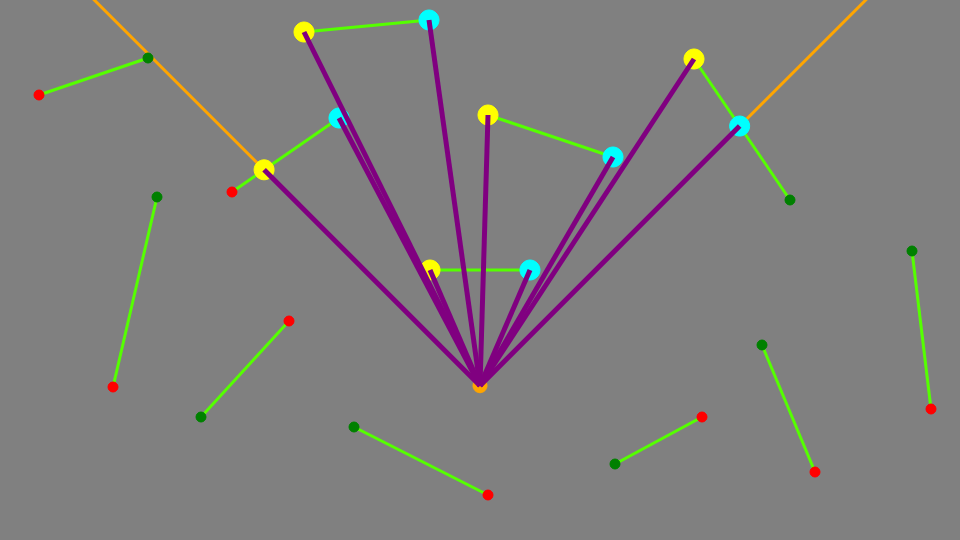
\includegraphics[width=0.7\textwidth,height=\textheight]{../img/New_rays_intersections_more.png}\strut
\end{minipage}\tabularnewline
\begin{minipage}[t]{0.97\columnwidth}\centering
Visualisation des obstacles intersectant avec les vecteurs de champ de
vision\strut
\end{minipage}\tabularnewline
\begin{minipage}[t]{0.97\columnwidth}\centering
(jaune pour l'extrémité gauche de l'obstacle et bleu pour l'extrémité
droite)\strut
\end{minipage}\tabularnewline
\bottomrule
\end{longtable}

D'abord on s'assure que \(\vec{p}\) soit bien à la gauche de \(\vec{h}\)
; dans le cas contraire, on inverse les données. Ensuite, on vérifie si
l'obstacle croise un des vecteurs du champ de vision. Si c'est le cas,
on définit à nouveau un des vecteurs pour qu'on n'ait seulement la
tranche de l'obstacle qui se trouve à l'intérieur du champ de vision.

\begin{Shaded}
\begin{Highlighting}[]
\KeywordTok{function} \AttributeTok{processFOV}\NormalTok{() }\OperatorTok{\{}
    \CommentTok{// make sure v1 is always to the left of v2}
    \ControlFlowTok{if}\NormalTok{ (}\OperatorTok{!}\AttributeTok{isClockwiseOrder}\NormalTok{(}\KeywordTok{this}\NormalTok{.}\AttributeTok{p}\OperatorTok{,} \KeywordTok{this}\NormalTok{.}\AttributeTok{h}\NormalTok{)) }\OperatorTok{\{}
        \KeywordTok{let}\NormalTok{ vtemp }\OperatorTok{=} \KeywordTok{this}\NormalTok{.}\AttributeTok{p}\OperatorTok{;}
        \KeywordTok{this}\NormalTok{.}\AttributeTok{p} \OperatorTok{=} \KeywordTok{this}\NormalTok{.}\AttributeTok{h}\OperatorTok{;}
        \KeywordTok{this}\NormalTok{.}\AttributeTok{h} \OperatorTok{=}\NormalTok{ vtemp}\OperatorTok{;}
    \OperatorTok{\}}

    \CommentTok{//  redefine wall if it intersects with LEFT fov ray}
    \ControlFlowTok{if}\NormalTok{ (}\OperatorTok{!}\AttributeTok{isClockwiseOrder}\NormalTok{(}\VariableTok{player}\NormalTok{.}\VariableTok{fov}\NormalTok{.}\VariableTok{v1}\NormalTok{.}\AttributeTok{dir}\OperatorTok{,} \KeywordTok{this}\NormalTok{.}\AttributeTok{p}\NormalTok{) }\OperatorTok{&&}
            \AttributeTok{isClockwiseOrder}\NormalTok{(}\VariableTok{player}\NormalTok{.}\VariableTok{fov}\NormalTok{.}\VariableTok{v1}\NormalTok{.}\AttributeTok{dir}\OperatorTok{,} \KeywordTok{this}\NormalTok{.}\AttributeTok{h}\NormalTok{)) }\OperatorTok{\{}
        \KeywordTok{this}\NormalTok{.}\AttributeTok{p} \OperatorTok{=} \AttributeTok{intersectionFovW}\NormalTok{(}\VariableTok{player}\NormalTok{.}\VariableTok{fov}\NormalTok{.}\AttributeTok{v1}\OperatorTok{,} \KeywordTok{this}\NormalTok{)}\OperatorTok{;}
        \KeywordTok{this}\NormalTok{.}\VariableTok{p}\NormalTok{.}\AttributeTok{x} \OperatorTok{-=} \VariableTok{player}\NormalTok{.}\VariableTok{pos}\NormalTok{.}\AttributeTok{x}\OperatorTok{;}
        \KeywordTok{this}\NormalTok{.}\VariableTok{p}\NormalTok{.}\AttributeTok{y} \OperatorTok{-=} \VariableTok{player}\NormalTok{.}\VariableTok{pos}\NormalTok{.}\AttributeTok{y}\OperatorTok{;}
    \OperatorTok{\}}

    \CommentTok{//  redefine wall if it intersects with RIGHT fov ray}
    \ControlFlowTok{if}\NormalTok{ (}\OperatorTok{!}\AttributeTok{isClockwiseOrder}\NormalTok{(}\VariableTok{player}\NormalTok{.}\VariableTok{fov}\NormalTok{.}\VariableTok{v2}\NormalTok{.}\AttributeTok{dir}\OperatorTok{,} \KeywordTok{this}\NormalTok{.}\AttributeTok{p}\NormalTok{) }\OperatorTok{&&}
            \AttributeTok{isClockwiseOrder}\NormalTok{(}\VariableTok{player}\NormalTok{.}\VariableTok{fov}\NormalTok{.}\VariableTok{v2}\NormalTok{.}\AttributeTok{dir}\OperatorTok{,} \KeywordTok{this}\NormalTok{.}\AttributeTok{h}\NormalTok{)) }\OperatorTok{\{}
        \KeywordTok{this}\NormalTok{.}\AttributeTok{h} \OperatorTok{=} \AttributeTok{intersectionFovW}\NormalTok{(}\VariableTok{player}\NormalTok{.}\VariableTok{fov}\NormalTok{.}\AttributeTok{v2}\OperatorTok{,} \KeywordTok{this}\NormalTok{)}\OperatorTok{;}
        \KeywordTok{this}\NormalTok{.}\VariableTok{h}\NormalTok{.}\AttributeTok{x} \OperatorTok{-=} \VariableTok{player}\NormalTok{.}\VariableTok{pos}\NormalTok{.}\AttributeTok{x}\OperatorTok{;}
        \KeywordTok{this}\NormalTok{.}\VariableTok{h}\NormalTok{.}\AttributeTok{y} \OperatorTok{-=} \VariableTok{player}\NormalTok{.}\VariableTok{pos}\NormalTok{.}\AttributeTok{y}\OperatorTok{;}
    \OperatorTok{\}}
    \ControlFlowTok{return} \KeywordTok{true}\OperatorTok{;}
\OperatorTok{\}}
\end{Highlighting}
\end{Shaded}

\hypertarget{impluxe9mentation}{%
\section{Implémentation}\label{impluxe9mentation}}

\hypertarget{calculs-de-projection-du-2d-au-3d}{%
\subsection{Calculs de projection du 2D au
3D}\label{calculs-de-projection-du-2d-au-3d}}

Maintenant qu'on a toutes les données nécessaires, on peut enfin
réaliser les calculs qui conduiront à une perspective 3D. On va prendre
les vecteurs \(\vec{p}\) et \(\vec{h}\) ainsi que le vecteur directeur
du joueur (celui qui indique son orientation) pour ensuite les
normaliser afin de pouvoir travailler avec leurs valeurs unitaires et ne
plus devoir se soucier de leur norme.

On appliquera ensuite la formule de l'angle entre deux vecteurs. L'angle
\texttt{v1xangle} correspond à l'angle entre le vecteur \(\vec{p}\) et
le vecteur directeur du joueur. L'angle \texttt{v2xangle} correspond à
celui entre \(\vec{p}\) et \(\vec{h}\). Les angles sont calculés ainsi
pour qu'on ait des valeurs allant du négatif au positif. On a un angle
relatif entre les vecteurs \(\vec{p}\) et \(\vec{h}\), qu'on dénote
respectivement \(\angle{p}\) et \(\angle{h}\). On a donc \(\angle{p}\)
qui est relatif au vecteur directeur du joueur ainsi que \(\angle{h}\)
qui n'est qu'une addition de \(\angle{p}\) et l'angle relatif entre les
deux.

Finalement, on définit les variables pour chacun des coins du polygone
qui sera généré pour dessiner l'obstacle. On calcule \texttt{x1} et
\texttt{x2} avec une proportion entre l'angle calculé précédemment et sa
place relative sur l'écran et \texttt{h1} et \texttt{h2} sont calculés
grâce à la fonction \texttt{calculateHeight()} dont je vais parler dans
la prochaine section.

\begin{Shaded}
\begin{Highlighting}[]
\KeywordTok{function} \AttributeTok{calculate3D}\NormalTok{() }\OperatorTok{\{}
    \KeywordTok{const}\NormalTok{ fovamount }\OperatorTok{=} \VariableTok{player}\NormalTok{.}\VariableTok{fov}\NormalTok{.}\AttributeTok{xamount}\OperatorTok{;}

    \KeywordTok{this}\NormalTok{.}\AttributeTok{p} \OperatorTok{=} \AttributeTok{vectorNormalize}\NormalTok{(}\KeywordTok{this}\NormalTok{.}\AttributeTok{p}\NormalTok{)}\OperatorTok{;}
    \KeywordTok{this}\NormalTok{.}\AttributeTok{h} \OperatorTok{=} \AttributeTok{vectorNormalize}\NormalTok{(}\KeywordTok{this}\NormalTok{.}\AttributeTok{h}\NormalTok{)}\OperatorTok{;}
    \KeywordTok{const}\NormalTok{ dir }\OperatorTok{=} \AttributeTok{vectorNormalize}\NormalTok{(}\VariableTok{player}\NormalTok{.}\AttributeTok{dir}\OperatorTok{,}
                    \VariableTok{Math}\NormalTok{.}\AttributeTok{sqrt}\NormalTok{((}\VariableTok{player}\NormalTok{.}\VariableTok{dir}\NormalTok{.}\AttributeTok{y}\NormalTok{) }\OperatorTok{**} \DecValTok{2} \OperatorTok{+}\NormalTok{ (}\VariableTok{player}\NormalTok{.}\VariableTok{dir}\NormalTok{.}\AttributeTok{x}\NormalTok{) }\OperatorTok{**} \DecValTok{2}\NormalTok{))}\OperatorTok{;}
    \KeywordTok{let}\NormalTok{ v1xangle }\OperatorTok{=} \VariableTok{Math}\NormalTok{.}\AttributeTok{acos}\NormalTok{(}\AttributeTok{vectorDotProduct}\NormalTok{(}\KeywordTok{this}\NormalTok{.}\AttributeTok{p}\OperatorTok{,}\NormalTok{ dir))}\OperatorTok{;}
    \KeywordTok{let}\NormalTok{ v2xangle }\OperatorTok{=} \VariableTok{Math}\NormalTok{.}\AttributeTok{acos}\NormalTok{(}\AttributeTok{vectorDotProduct}\NormalTok{(}\KeywordTok{this}\NormalTok{.}\AttributeTok{h}\OperatorTok{,} \KeywordTok{this}\NormalTok{.}\AttributeTok{p}\NormalTok{))}\OperatorTok{;}

    \CommentTok{// correct sign depending on side of v1/v2        }
    \ControlFlowTok{if}\NormalTok{ (}\OperatorTok{!}\AttributeTok{isClockwiseOrder}\NormalTok{(dir}\OperatorTok{,} \KeywordTok{this}\NormalTok{.}\AttributeTok{p}\NormalTok{)) v1xangle }\OperatorTok{=} \OperatorTok{-}\NormalTok{v1xangle}\OperatorTok{;} 
    \ControlFlowTok{if}\NormalTok{ (}\OperatorTok{!}\AttributeTok{isClockwiseOrder}\NormalTok{(}\KeywordTok{this}\NormalTok{.}\AttributeTok{p}\OperatorTok{,} \KeywordTok{this}\NormalTok{.}\AttributeTok{h}\NormalTok{)) v2xangle }\OperatorTok{=} \OperatorTok{-}\NormalTok{v2xangle}\OperatorTok{;}

\NormalTok{    v2xangle }\OperatorTok{=}\NormalTok{ v2xangle }\OperatorTok{+}\NormalTok{ v1xangle}\OperatorTok{;} \CommentTok{// make v2 relative to v1}

    \KeywordTok{this}\NormalTok{.}\VariableTok{p}\NormalTok{.}\AttributeTok{dist} \OperatorTok{*=} \VariableTok{Math}\NormalTok{.}\AttributeTok{cos}\NormalTok{(v1xangle)}\OperatorTok{;}
    \KeywordTok{this}\NormalTok{.}\AttributeTok{x1} \OperatorTok{=} \AttributeTok{degrees}\NormalTok{(v1xangle) }\OperatorTok{*} \VariableTok{canvas}\NormalTok{.}\AttributeTok{width}\NormalTok{ / fovamount}\OperatorTok{;}
    \KeywordTok{this}\NormalTok{.}\AttributeTok{h1} \OperatorTok{=} \KeywordTok{this}\NormalTok{.}\AttributeTok{calculateHeight}\NormalTok{(}\KeywordTok{this}\NormalTok{.}\AttributeTok{p}\NormalTok{)}\OperatorTok{;}

    \KeywordTok{this}\NormalTok{.}\VariableTok{h}\NormalTok{.}\AttributeTok{dist} \OperatorTok{*=} \VariableTok{Math}\NormalTok{.}\AttributeTok{cos}\NormalTok{(v2xangle)}\OperatorTok{;}
    \KeywordTok{this}\NormalTok{.}\AttributeTok{x2} \OperatorTok{=} \AttributeTok{degrees}\NormalTok{(v2xangle) }\OperatorTok{*} \VariableTok{canvas}\NormalTok{.}\AttributeTok{width}\NormalTok{ / fovamount}\OperatorTok{;}
    \KeywordTok{this}\NormalTok{.}\AttributeTok{h2} \OperatorTok{=} \KeywordTok{this}\NormalTok{.}\AttributeTok{calculateHeight}\NormalTok{(}\KeywordTok{this}\NormalTok{.}\AttributeTok{h}\NormalTok{)}\OperatorTok{;}

    \ControlFlowTok{if}\NormalTok{ (}\KeywordTok{this}\NormalTok{.}\AttributeTok{h1} \OperatorTok{>} \DecValTok{10000}\NormalTok{) }\KeywordTok{this}\NormalTok{.}\AttributeTok{h1} \OperatorTok{=} \DecValTok{10000}\OperatorTok{;}
    \ControlFlowTok{if}\NormalTok{ (}\KeywordTok{this}\NormalTok{.}\AttributeTok{h2} \OperatorTok{>} \DecValTok{10000}\NormalTok{) }\KeywordTok{this}\NormalTok{.}\AttributeTok{h2} \OperatorTok{=} \DecValTok{10000}\OperatorTok{;}
\OperatorTok{\}}
\end{Highlighting}
\end{Shaded}

\hypertarget{calculer-la-taille-relative-dun-obstacle-dans-le-champ-de-vision}{%
\subsection{Calculer la taille relative d'un obstacle dans le champ de
vision}\label{calculer-la-taille-relative-dun-obstacle-dans-le-champ-de-vision}}

Après avoir calculé la distance entre le joueur et un point sur un
obstacle, on peut alors déterminer la hauteur que cette tranche
d'obstacle prendra sur la perspective 3D.

Les valeurs dont on a besoin sont~: \emph{dist} la distance calculée
précédemment grâce à la fonction \texttt{intersection()}, \(h_0\) la
différence entre le bas de l'obstacle et la hauteur du joueur, \(h_1\)
la différence entre le haut de l'obstacle et la hauteur du joueur,
\(\mathrm{floor}\) la différence entre la hauteur du joueur et le sol,
\(canvas_{height}\) la hauteur en pixels de l'écran en perspective 3D et
\(FOV_y\) la valeur verticale maximale du champ de vision. Pour mieux
illustrer ces points, on les représentera sous forme de vecteurs, mais
on n'a seulement besoin des valeurs verticales, car la valeur
horizontale est la même. La hauteur du joueur ainsi que celle du haut et
le bas de chaque obstacle sont prédéfinies et peuvent être modifiées
librement.

\begin{longtable}[]{@{}c@{}}
\toprule
\endhead
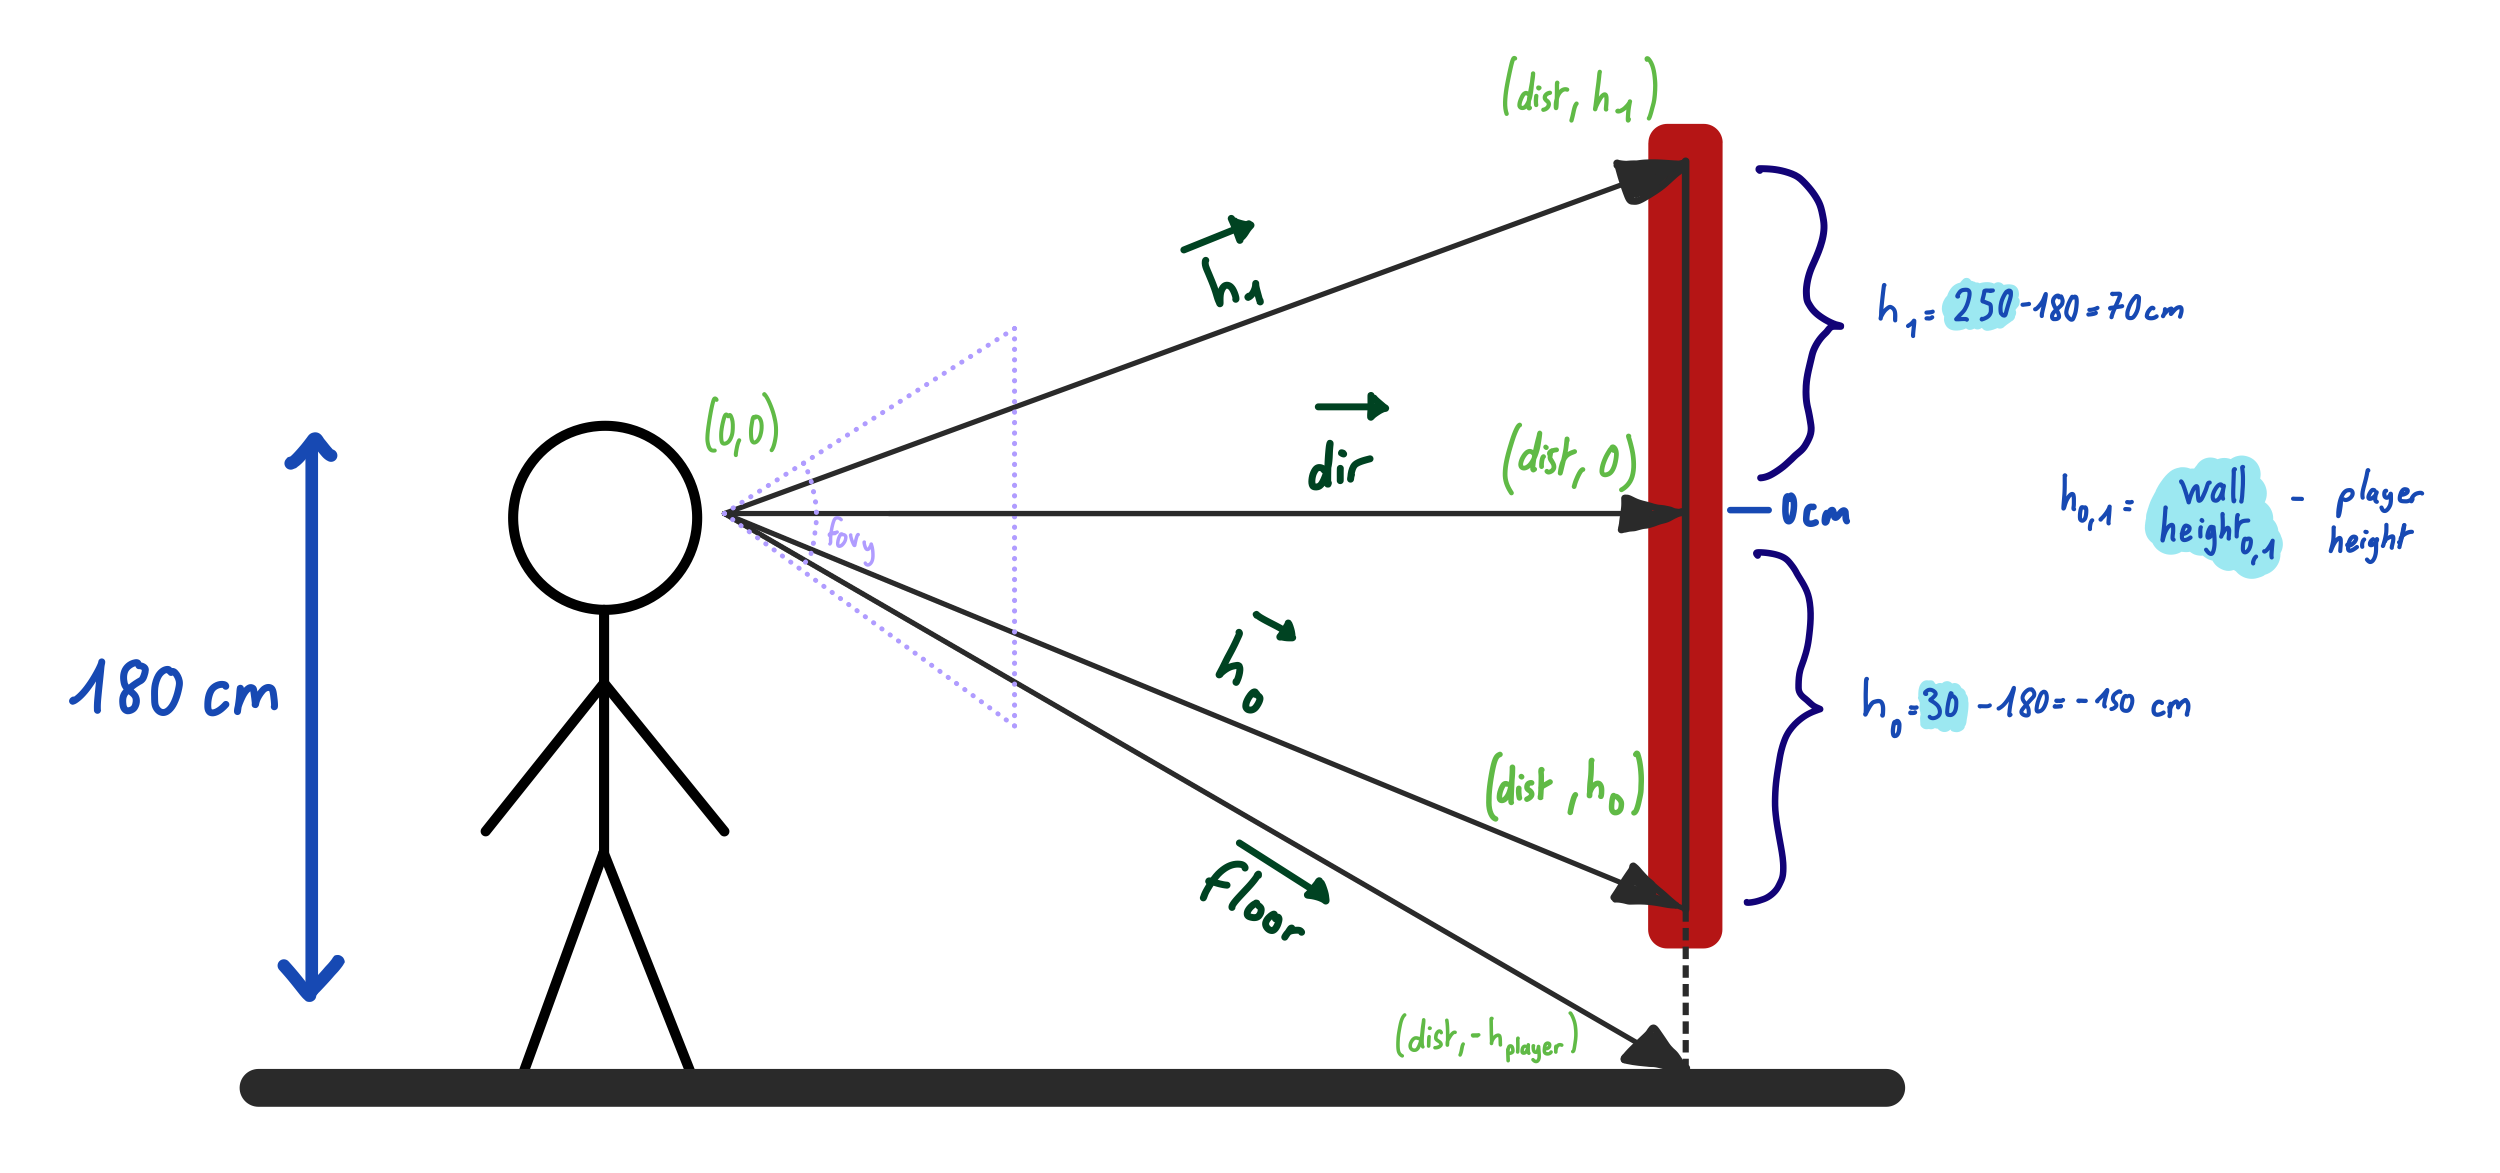
\includegraphics[width=0.8\textwidth,height=\textheight]{../img/Drawings/new_vertical_raycast_drawing.png}\tabularnewline
Représentation schématique des valeurs\tabularnewline
\bottomrule
\end{longtable}

Ainsi, on peut calculer la proportion entre la hauteur de ces points et
la hauteur relative à l'écran en perspective 3D grâce aux formules
suivantes~:

\[
\mathrm{floor{_{height}}} = \frac{\mathrm{floor{_y}\cdot \mathrm{canvas_{height}}}}
                                 {\tan{(FOV_y)} \cdot dist} \quad
\mathrm{h_0{_{height}}} = \frac{\mathrm{h_0{_y} \cdot \mathrm{canvas_{height}}}}
                               {\tan{(FOV_y)} \cdot dist} \quad
\mathrm{h_1{_{height}}} = \frac{\mathrm{h_1{_y} \cdot \mathrm{canvas_{height}}}}
                               {\tan{(FOV_y)} \cdot dist}
\]

Ensuite, on peut utiliser une proportion entre l'angle et la hauteur de
l'écran de la perspective 3D. La fonction \emph{calculateHeight()}
retourne enfin ces valeurs calculées par cette proportion.

Au moment de rendre ce projet comme travail de Maturité, cette partie de
mon programme était plus complexe que nécessaire, car j'ai essayé de
trouver des mesures grâce aux angles. Ceci donnait une projection qui
paraissaît à première vue bonne, mais on se rendait vite compte que
quelque chose était faux. Finalement, la proportionnalité entre les
différentes hauteurs donne un calcul plus simple et des hauteurs qui
ressemblent à ce qu'on percevrait de nos propres yeux

\begin{Shaded}
\begin{Highlighting}[]
\KeywordTok{function} \AttributeTok{calculateHeight}\NormalTok{(v) }\OperatorTok{\{}
    \KeywordTok{const}\NormalTok{ h0 }\OperatorTok{=} \AttributeTok{vectorCreate}\NormalTok{(}\VariableTok{v}\NormalTok{.}\AttributeTok{dist}\OperatorTok{,} \KeywordTok{this}\NormalTok{.}\AttributeTok{height0} \OperatorTok{-} \VariableTok{player}\NormalTok{.}\AttributeTok{height}\NormalTok{)}\OperatorTok{;}
    \KeywordTok{const}\NormalTok{ h1 }\OperatorTok{=} \AttributeTok{vectorCreate}\NormalTok{(}\VariableTok{v}\NormalTok{.}\AttributeTok{dist}\OperatorTok{,} \KeywordTok{this}\NormalTok{.}\AttributeTok{height1} \OperatorTok{-} \VariableTok{player}\NormalTok{.}\AttributeTok{height}\NormalTok{)}\OperatorTok{;}
    \KeywordTok{const}\NormalTok{ floor }\OperatorTok{=} \AttributeTok{vectorCreate}\NormalTok{(}\VariableTok{v}\NormalTok{.}\AttributeTok{dist}\OperatorTok{,} \OperatorTok{-}\VariableTok{player}\NormalTok{.}\AttributeTok{height}\NormalTok{)}\OperatorTok{;} 

    \ControlFlowTok{return} \OperatorTok{\{}
        \StringTok{'floor'}\OperatorTok{:}\NormalTok{ (}\VariableTok{floor}\NormalTok{.}\AttributeTok{y} \OperatorTok{*} \VariableTok{canvas}\NormalTok{.}\AttributeTok{height}\NormalTok{)}
\NormalTok{                    / (}\VariableTok{Math}\NormalTok{.}\AttributeTok{tan}\NormalTok{(}\AttributeTok{radians}\NormalTok{(}\VariableTok{player}\NormalTok{.}\VariableTok{fov}\NormalTok{.}\AttributeTok{yamount}\NormalTok{)) }\OperatorTok{*} \VariableTok{v}\NormalTok{.}\AttributeTok{dist}\NormalTok{)}\OperatorTok{,}
        \StringTok{'h0'}\OperatorTok{:}\NormalTok{    (}\VariableTok{h0}\NormalTok{.}\AttributeTok{y} \OperatorTok{*} \VariableTok{canvas}\NormalTok{.}\AttributeTok{height}\NormalTok{)}
\NormalTok{                    / (}\VariableTok{Math}\NormalTok{.}\AttributeTok{tan}\NormalTok{(}\AttributeTok{radians}\NormalTok{(}\VariableTok{player}\NormalTok{.}\VariableTok{fov}\NormalTok{.}\AttributeTok{yamount}\NormalTok{)) }\OperatorTok{*} \VariableTok{v}\NormalTok{.}\AttributeTok{dist}\NormalTok{)}\OperatorTok{,}
        \StringTok{'h1'}\OperatorTok{:}\NormalTok{    (}\VariableTok{h1}\NormalTok{.}\AttributeTok{y} \OperatorTok{*} \VariableTok{canvas}\NormalTok{.}\AttributeTok{height}\NormalTok{)}
\NormalTok{                    / (}\VariableTok{Math}\NormalTok{.}\AttributeTok{tan}\NormalTok{(}\AttributeTok{radians}\NormalTok{(}\VariableTok{player}\NormalTok{.}\VariableTok{fov}\NormalTok{.}\AttributeTok{yamount}\NormalTok{)) }\OperatorTok{*} \VariableTok{v}\NormalTok{.}\AttributeTok{dist}\NormalTok{)}\OperatorTok{,}
        \StringTok{'sat'}\OperatorTok{:} \DecValTok{1}\OperatorTok{,}
        \StringTok{'dist'}\OperatorTok{:} \VariableTok{v}\NormalTok{.}\AttributeTok{dist}
    \OperatorTok{\};}
\OperatorTok{\}}
\end{Highlighting}
\end{Shaded}

\hypertarget{tri-des-obstacles}{%
\subsection{Tri des obstacles}\label{tri-des-obstacles}}

Actuellement, on a une liste des obstacles que l'on doit dessiner dans
un ordre au hasard. Sans traitement de cette liste, on peut se retrouver
avec un rendu comme le suivant.

\begin{longtable}[]{@{}cc@{}}
\toprule
\endhead
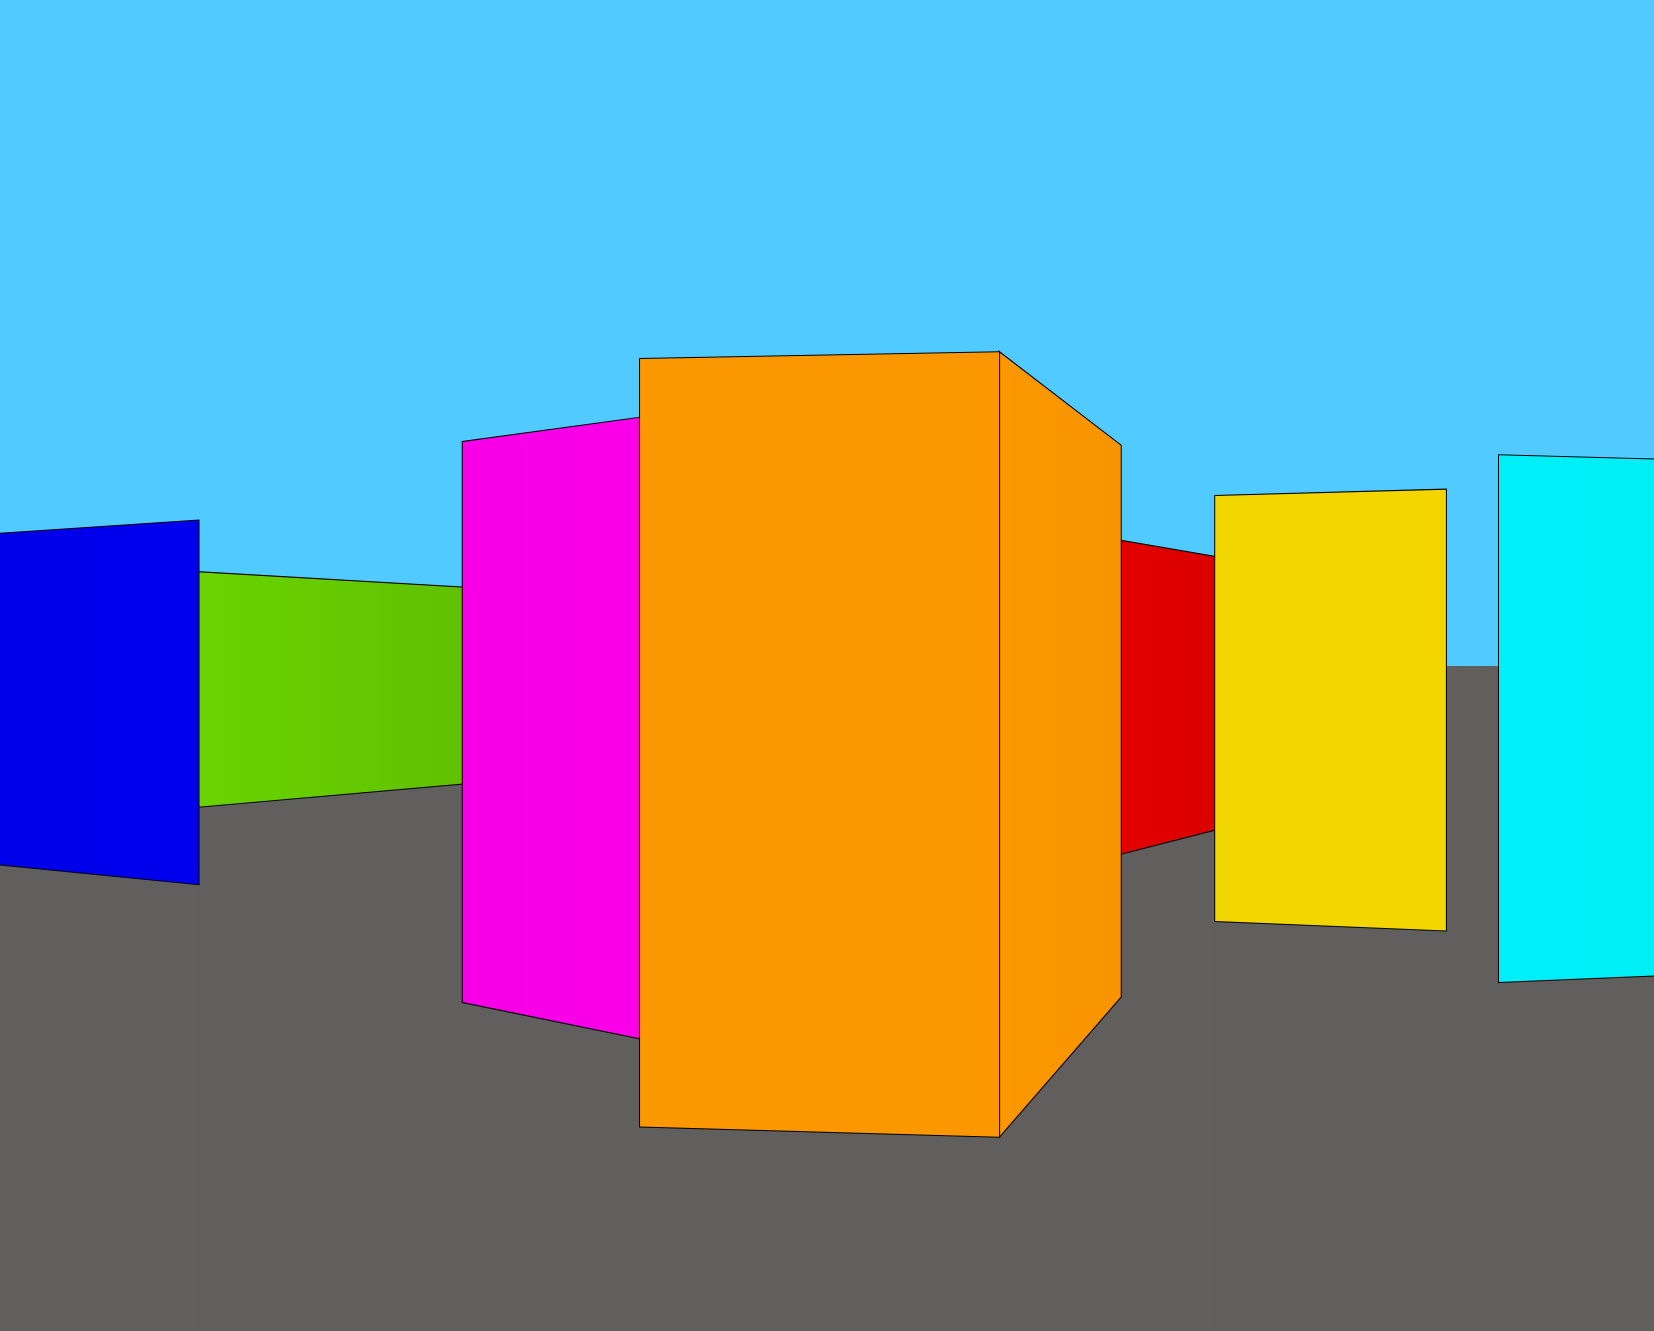
\includegraphics[width=0.4\textwidth,height=\textheight]{../img/CoverPic/SortedMain.png}
&
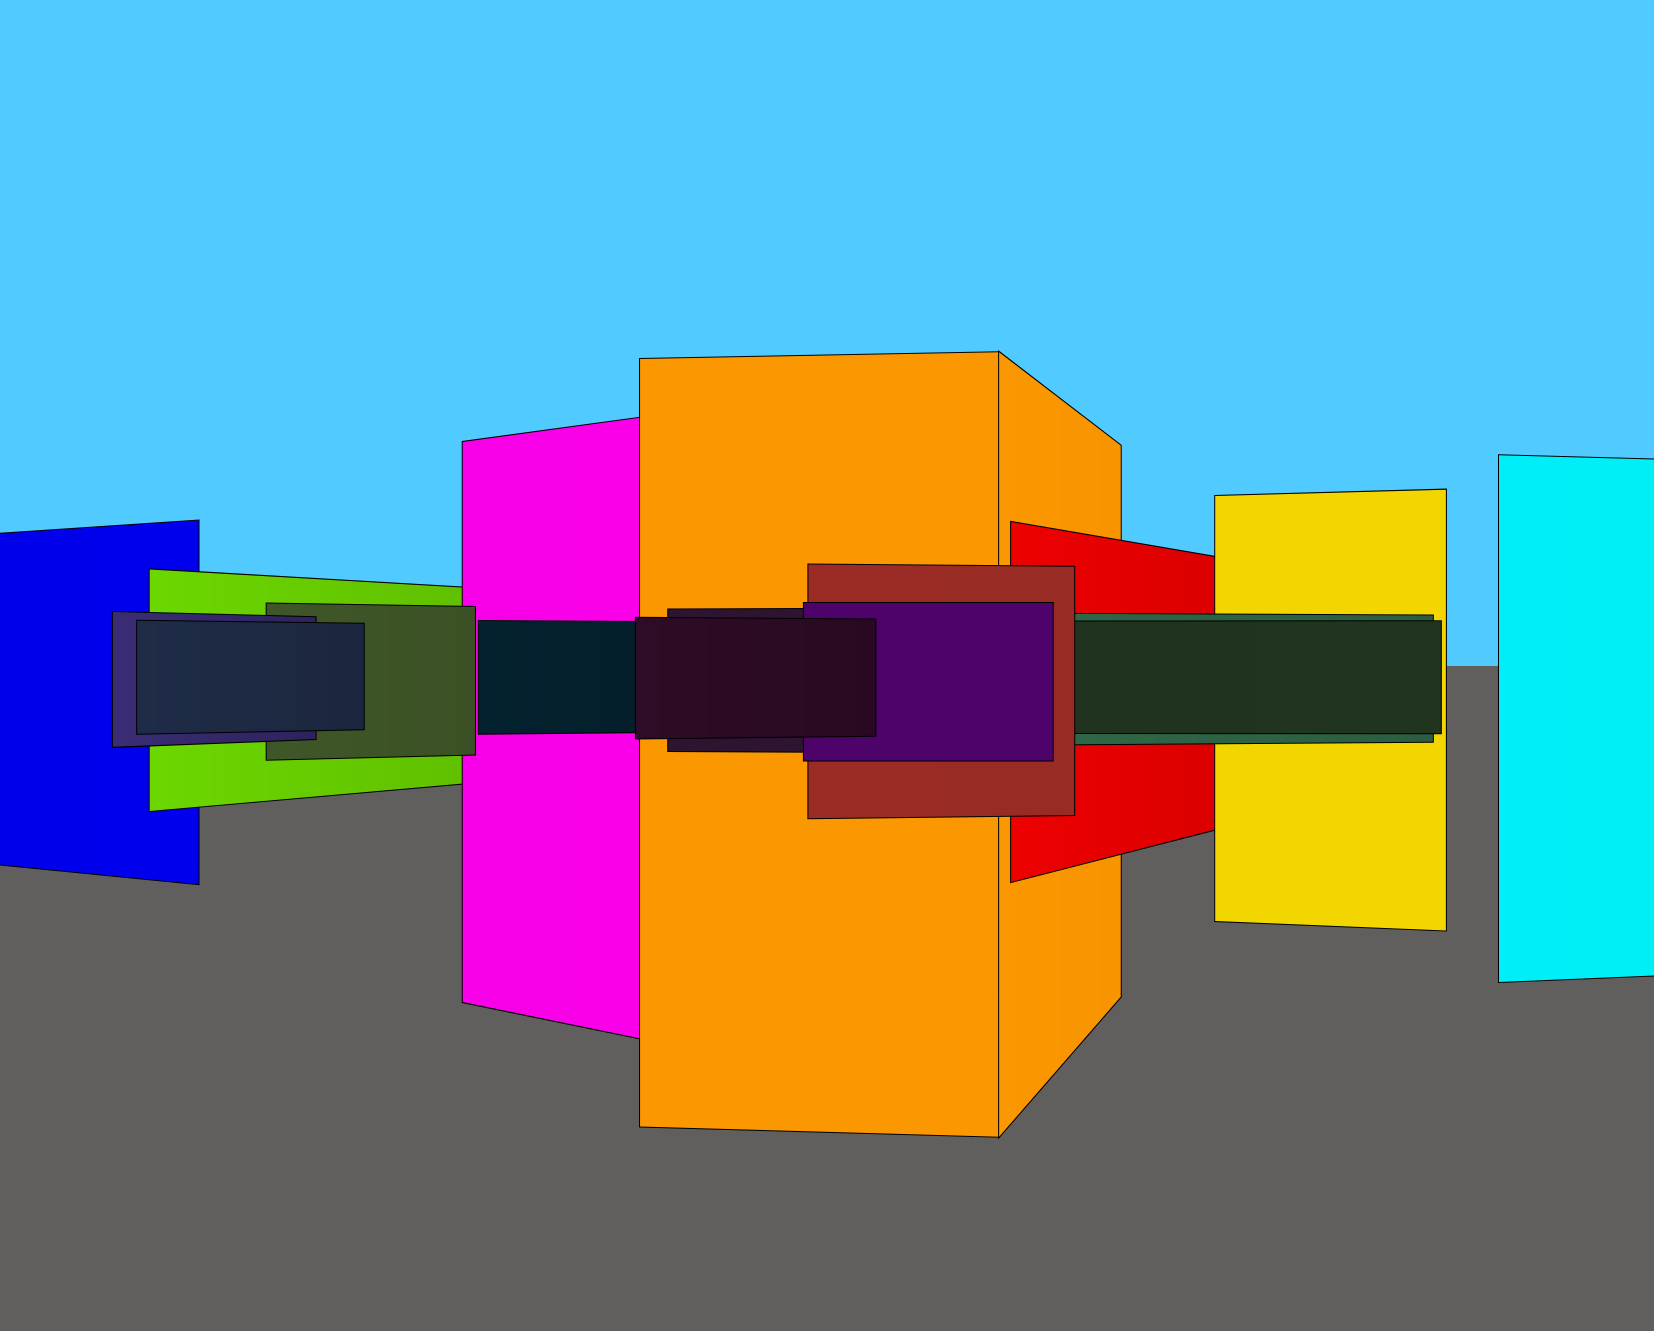
\includegraphics[width=0.4\textwidth,height=\textheight]{../img/CoverPic/UnsortedMain.png}\tabularnewline
Rendu avec tri des obstacles & Rendu sans tri\tabularnewline
\bottomrule
\end{longtable}

On a donc besoin de trier ces obstacles en fonction de leur distance par
rapport au joueur. Ceci tient en compte qu'il faut pouvoir déterminer si
un obstacle est derrière ou devant un autre par rapport au joueur. On
n'a pas non plus de valeur unique à comparer, car chaque obstacle
possède deux coordonnées x et y et il faut que tout soit calculé
relativement au joueur.

\emph{Un ensemble d'ordre total} est un ensemble dont tous les éléments
sont comparables entre eux. Par exemple, un ensemble de nombres qui deux
a deux peuvent tous être comparés pour les ordonner du petit au plus
grand.

Dans notre cas, l'ensemble d'obstacles n'est pas d'ordre total, car il
peut exister deux paires, où aucun des deux est devant l'autre. En
réalité, cet ensemble s'appelle un \emph{Ensemble Partiellement Ordonné}
(ou \emph{POSET} en anglais pour \emph{Partially Ordered Set}). Pour
effectuer un tri, on utilise ce qu'on appelle un \emph{graphe}. C'est
une manière de représenter la hiérarchie des relations entre des objets.
Chaque point, appelé un \emph{sommet}, représente un objet, et chacun de
ces sommets est lié par ce qu'on appelle une \emph{arête}. En mettant en
relation chaque obstacle dans un graphe, la présentation de celui-ci
ressemble à une sorte d'arbre.

\begin{longtable}[]{@{}cc@{}}
\toprule
\endhead
\begin{minipage}[t]{0.47\columnwidth}\centering
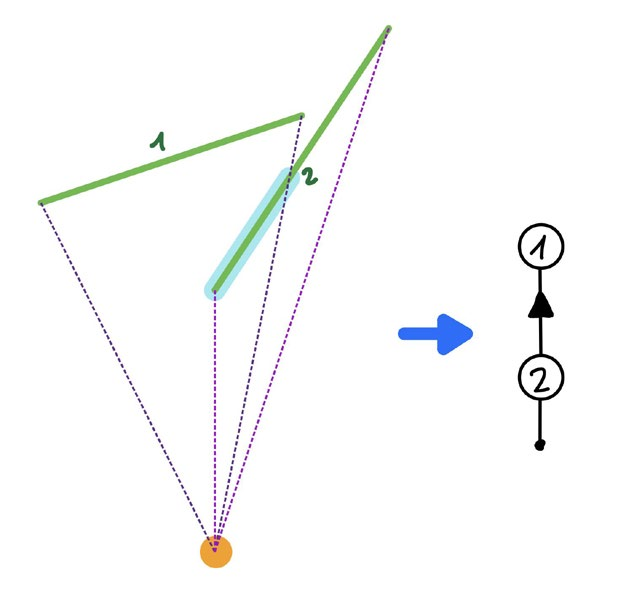
\includegraphics[width=\textwidth,height=2.08333in]{../img/Graphs/graph_overlap1.png}\strut
\end{minipage} & \begin{minipage}[t]{0.47\columnwidth}\centering
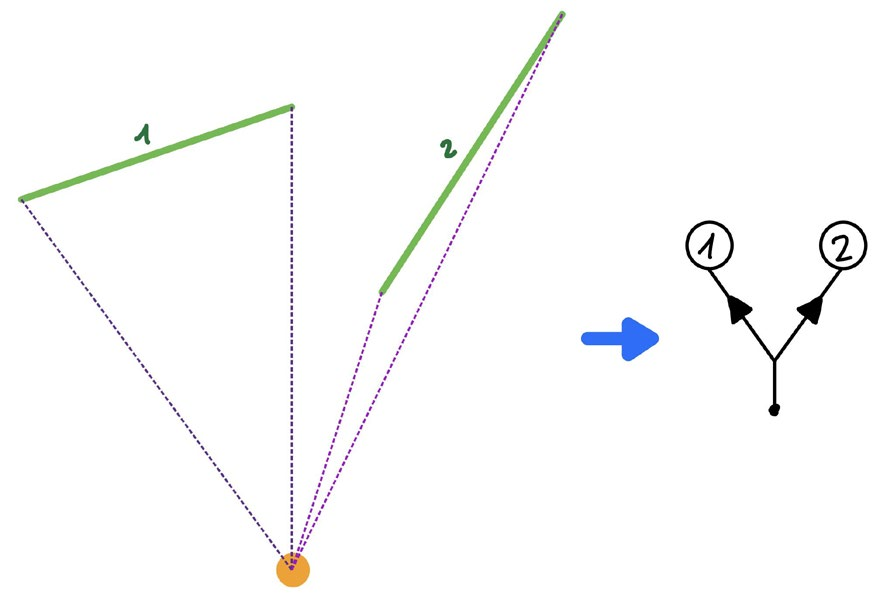
\includegraphics[width=\textwidth,height=2.08333in]{../img/Graphs/graph_overlap2.png}\strut
\end{minipage}\tabularnewline
\begin{minipage}[t]{0.47\columnwidth}\centering
Deux obstacles qui ont une relation entre eux par rapport au
joueur\strut
\end{minipage} & \begin{minipage}[t]{0.47\columnwidth}\centering
Deux obstacles qui n'ont aucune relation entre eux par rapport au
joueur\strut
\end{minipage}\tabularnewline
\bottomrule
\end{longtable}

Dans les images ci-dessus figurent deux exemples avec une paire
d'obstacles ainsi que leur représentation sous forme de graphe. À
gauche, l'obstacle 2 apparaît devant l'obstacle 1, donc il est placé
avant le premier dans le graphe. À droite, aucun des deux n'est devant
ou derrière l'autre, donc on va les représenter par deux arêtes
divergentes, appelées branches, sur le graphe.

\begin{longtable}[]{@{}c@{}}
\toprule
\endhead
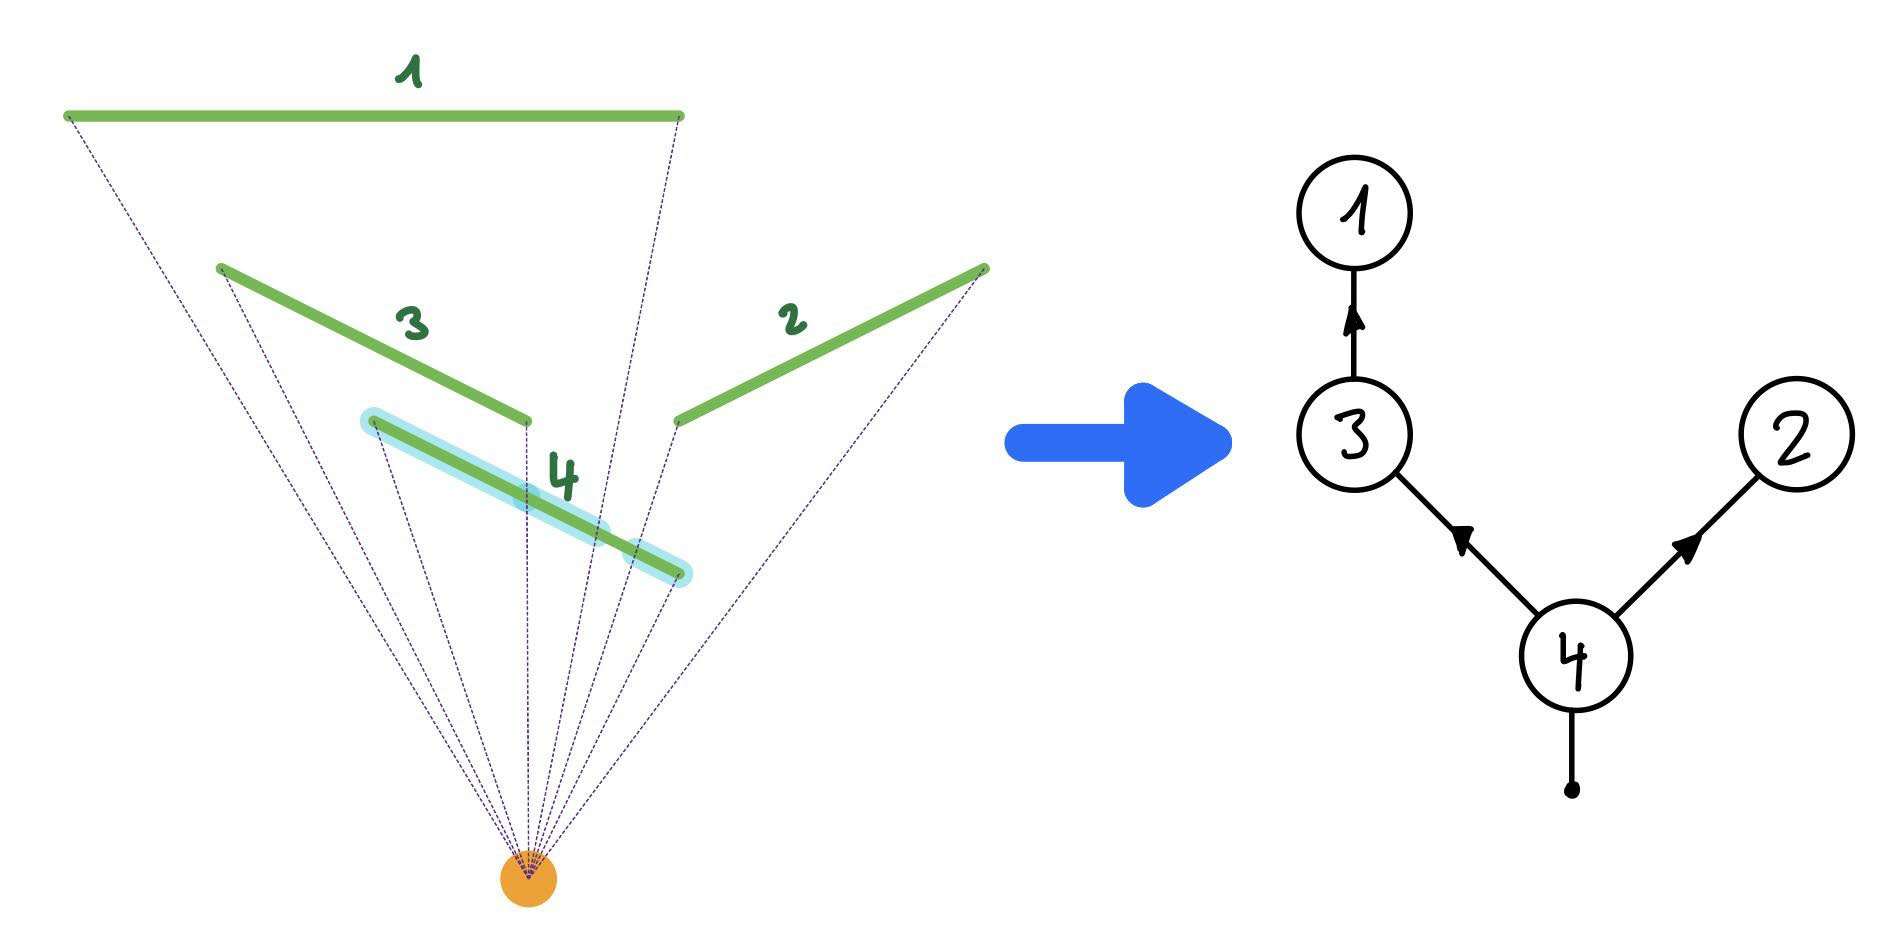
\includegraphics[width=\textwidth,height=2.08333in]{../img/Graphs/graph_overlap3.png}\tabularnewline
Cas d'un graphe avec plusieurs branches\tabularnewline
\bottomrule
\end{longtable}

Dans l'image ci-dessus, les deux cas sont fusionnés. On remarque que
l'obstacle 4 paraît devant tous les autres, sans que ceux-ci aient de
relation entre eux.

\hypertarget{cruxe9ation-du-graphe}{%
\subsubsection{Création du graphe}\label{cruxe9ation-du-graphe}}

\hypertarget{crituxe8res-de-comparaison-entre-deux-obstacles}{%
\paragraph{Critères de comparaison entre deux
obstacles}\label{crituxe8res-de-comparaison-entre-deux-obstacles}}

Afin de créer les graphes, il faut une fonction qui peut comparer deux
obstacles et déterminer s'ils sont l'un devant l'autre ou pas. Cette
fonction s'appelle \texttt{v1HigherThanv2()}. La comparaison doit se
faire de manière que toutes les possibilités de placement d'obstacles
soient pris en compte.

La version actuelle prend en compte trois cas.

\begin{longtable}[]{@{}ccc@{}}
\toprule
\begin{minipage}[b]{0.30\columnwidth}\centering
Cas 1\strut
\end{minipage} & \begin{minipage}[b]{0.30\columnwidth}\centering
Cas 2\strut
\end{minipage} & \begin{minipage}[b]{0.30\columnwidth}\centering
Cas 3\strut
\end{minipage}\tabularnewline
\midrule
\endhead
\begin{minipage}[t]{0.30\columnwidth}\centering
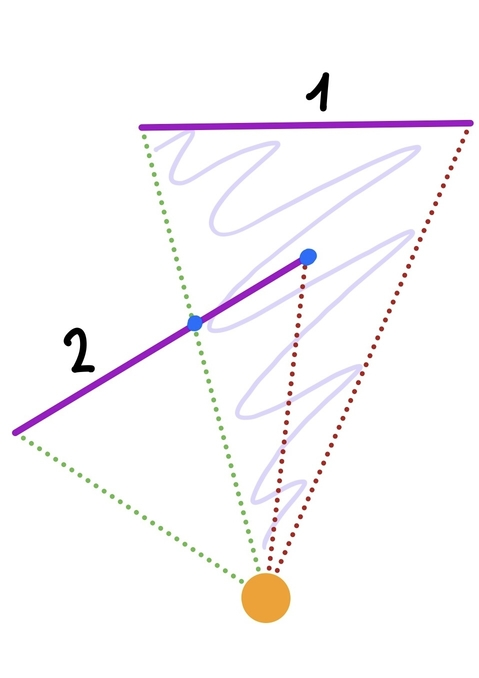
\includegraphics[width=\textwidth,height=1.5625in]{../img/Graphs/InsideTriangleResize.jpg}\strut
\end{minipage} & \begin{minipage}[t]{0.30\columnwidth}\centering
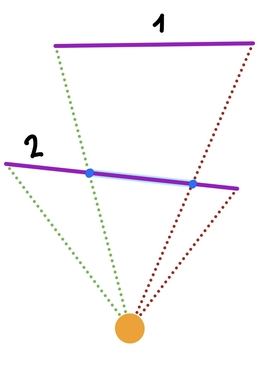
\includegraphics[width=\textwidth,height=1.5625in]{../img/Graphs/IntersectingResize.jpg}\strut
\end{minipage} & \begin{minipage}[t]{0.30\columnwidth}\centering
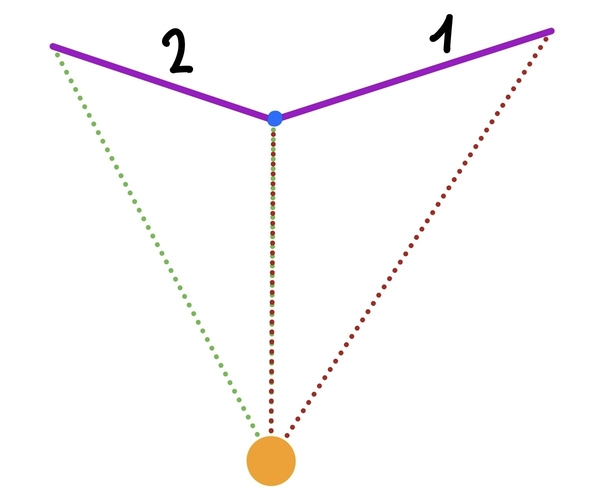
\includegraphics[width=\textwidth,height=1.5625in]{../img/Graphs/IsSameResize.jpg}\strut
\end{minipage}\tabularnewline
\begin{minipage}[t]{0.30\columnwidth}\centering
Une des extrémités d'un obstacle devant l'autre\strut
\end{minipage} & \begin{minipage}[t]{0.30\columnwidth}\centering
Un obstacle cachant l'autre\strut
\end{minipage} & \begin{minipage}[t]{0.30\columnwidth}\centering
Obstacles collés, mais pas superposés\strut
\end{minipage}\tabularnewline
\bottomrule
\end{longtable}

\textbf{Cas 1)} D'abord, il y a une vérification de si une des
extrémités de l'obstacle 2 se trouve devant l'autre. On peut faire ceci
en considérant que les deux extrémités de l'obstacle 1 ainsi que le
point où se situe le joueur forment un triangle. Ensuite, si le point de
l'obstacle 2 est effectivement à l'intérieur du triangle, alors on sait
que l'obstacle 2 est bien devant le 1.

\textbf{Cas 2)} On réalise aussi une vérification d'intersections entre
l'obstacle 2 et les vecteurs reliant le joueur à l'obstacle 1. Si c'est
le cas, ça veut dire que l'obstacle 2 est forcément devant le 1.

\textbf{Cas 3)} Finalement, on vérifie si les obstacles partagent des
extrémités entre eux, car ce cas ne retourne pas vrai dans les autres
vérifications. En implémentant cette partie du code, j'ai eu des
difficultés pour comparer les coordonnées de deux points, car il y a
comparaison de deux nombres décimaux.

\hypertarget{erreurs-de-pruxe9cision-des-points-flottants}{%
\paragraph{Erreurs de précision des points
flottants}\label{erreurs-de-pruxe9cision-des-points-flottants}}

L'ordinateur stocke ces nombres, qu'on appelle aussi \emph{points
flottants}, sous une notation scientifique en base 2. Bien que cette
manière nous offre la possibilité de travailler avec des décimales, elle
vient également avec certains problèmes qui sont les erreurs de
précision. En effet, l'addition de deux points flottants \(0.1 + 0.2\)
qui équivaudrait \(0.3\) normalement, ne donne pas le même résultat dans
un programme. Ceci est dû à la représentation de \(0.1\) et \(0.2\) qui
sont, selon l'ordinateur équivalent à, par exemple, \(0.100000001\) ou
\(0.20000012\). Ces nombres sont des arrondis qui sont malheureusement
nécessaires, car un ordinateur ne peut pas représenter ces nombres avec
une telle précision.

\begin{Shaded}
\begin{Highlighting}[]
\KeywordTok{const}\NormalTok{ EPSILON }\OperatorTok{=} \FloatTok{0.01}
\KeywordTok{function} \AttributeTok{isSame}\NormalTok{(v1}\OperatorTok{,}\NormalTok{ v2) }\OperatorTok{\{}
    \ControlFlowTok{return}  \VariableTok{Math}\NormalTok{.}\AttributeTok{abs}\NormalTok{(}\VariableTok{v1}\NormalTok{.}\AttributeTok{x} \OperatorTok{-} \VariableTok{v2}\NormalTok{.}\AttributeTok{x}\NormalTok{) }\OperatorTok{<}\NormalTok{ EPSILON }\OperatorTok{&&}
            \VariableTok{Math}\NormalTok{.}\AttributeTok{abs}\NormalTok{(}\VariableTok{v1}\NormalTok{.}\AttributeTok{y} \OperatorTok{-} \VariableTok{v2}\NormalTok{.}\AttributeTok{y}\NormalTok{) }\OperatorTok{<}\NormalTok{ EPSILON}
\OperatorTok{\}}
\end{Highlighting}
\end{Shaded}

Pour contrer ce problème, lorsqu'on veut vérifier l'égalité entre deux
points flottants, on prend la différence entre les deux et on vérifie si
celle-ci est plus petite qu'une certaine constante. Dans mon programme,
j'englobe cette comparaison sous la fonction \texttt{isSame()} qui
utilise une constante appelée \emph{Epsilon} qui vaut 0.01. Cette
fonction retourne vrai si la différence entre les coordonnées des deux
points donne un nombre inférieur à la constante. Ceci permet de survenir
au problème de précision, car on inclut une certaine marge d'erreur.

\begin{Shaded}
\begin{Highlighting}[]
\KeywordTok{function} \AttributeTok{v1HigherThanv2}\NormalTok{(w1}\OperatorTok{,}\NormalTok{ w2) }\OperatorTok{\{}
    \CommentTok{// CAS 3}
    \ControlFlowTok{if}\NormalTok{ (}\AttributeTok{isSame}\NormalTok{(}\AttributeTok{vectorMult}\NormalTok{(}\VariableTok{w1}\NormalTok{.}\AttributeTok{p}\OperatorTok{,} \VariableTok{w1}\NormalTok{.}\VariableTok{p}\NormalTok{.}\AttributeTok{dist}\NormalTok{)}\OperatorTok{,} \AttributeTok{vectorMult}\NormalTok{(}\VariableTok{w2}\NormalTok{.}\AttributeTok{h}\OperatorTok{,} \VariableTok{w2}\NormalTok{.}\VariableTok{h}\NormalTok{.}\AttributeTok{dist}\NormalTok{)) }\OperatorTok{||}
        \AttributeTok{isSame}\NormalTok{(}\AttributeTok{vectorMult}\NormalTok{(}\VariableTok{w1}\NormalTok{.}\AttributeTok{h}\OperatorTok{,} \VariableTok{w1}\NormalTok{.}\VariableTok{h}\NormalTok{.}\AttributeTok{dist}\NormalTok{)}\OperatorTok{,} \AttributeTok{vectorMult}\NormalTok{(}\VariableTok{w2}\NormalTok{.}\AttributeTok{p}\OperatorTok{,} \VariableTok{w2}\NormalTok{.}\VariableTok{p}\NormalTok{.}\AttributeTok{dist}\NormalTok{))) }\OperatorTok{\{}
        \ControlFlowTok{return} \KeywordTok{false}
    \OperatorTok{\}}

    \CommentTok{// CAS 1 et 2}
    \ControlFlowTok{return}  \AttributeTok{isIntersectionVectors}\NormalTok{(PltoW1P}\OperatorTok{,}\NormalTok{ W2ptoW2h}\OperatorTok{,} \VariableTok{w1}\NormalTok{.}\AttributeTok{index}\OperatorTok{,} \VariableTok{w2}\NormalTok{.}\AttributeTok{index}\NormalTok{) }\OperatorTok{||}
            \AttributeTok{isIntersectionVectors}\NormalTok{(PltoW1H}\OperatorTok{,}\NormalTok{ W2ptoW2h}\OperatorTok{,} \VariableTok{w1}\NormalTok{.}\AttributeTok{index}\OperatorTok{,} \VariableTok{w2}\NormalTok{.}\AttributeTok{index}\NormalTok{) }\OperatorTok{||}
            \AttributeTok{ptInTriangle}\NormalTok{(W2p}\OperatorTok{,} \VariableTok{player}\NormalTok{.}\AttributeTok{pos}\OperatorTok{,}\NormalTok{ W1p}\OperatorTok{,}\NormalTok{ W1h}\OperatorTok{,} \VariableTok{w1}\NormalTok{.}\AttributeTok{index}\OperatorTok{,} \VariableTok{w2}\NormalTok{.}\AttributeTok{index}\NormalTok{) }\OperatorTok{||}
            \AttributeTok{ptInTriangle}\NormalTok{(W2h}\OperatorTok{,} \VariableTok{player}\NormalTok{.}\AttributeTok{pos}\OperatorTok{,}\NormalTok{ W1p}\OperatorTok{,}\NormalTok{ W1h}\OperatorTok{,} \VariableTok{w1}\NormalTok{.}\AttributeTok{index}\OperatorTok{,} \VariableTok{w2}\NormalTok{.}\AttributeTok{index}\NormalTok{)}
\OperatorTok{\}}
\end{Highlighting}
\end{Shaded}

\hypertarget{comparer-tous-les-obstacles-entre-eux}{%
\subsubsection{Comparer tous les obstacles entre
eux}\label{comparer-tous-les-obstacles-entre-eux}}

Maintenant qu'on a établi une comparaison entre deux obstacles, on doit
pouvoir associer chacun d'entre eux ensemble et ainsi créer un graphe.
La fonction \texttt{wallsToGraph()} va associer chaque obstacle avec un
autre de manière que chaque paire soit unique. C'est une combinaison
dont l'ordre n'est pas important, car la comparaison avec la fonction
\texttt{v1HigherThanv2()} se fait dans les deux sens afin de savoir dans
quel ordre placer les obstacles dans le graphe. S'ils n'ont aucun lien
entre eux, on va les ajouter au graphe, mais en tant que sommets
individuels plutôt qu'une arête dans un sens.

\begin{Shaded}
\begin{Highlighting}[]
\KeywordTok{function} \AttributeTok{wallsToGraph}\NormalTok{(w) }\OperatorTok{\{}
    \ControlFlowTok{if}\NormalTok{ (}\VariableTok{w}\NormalTok{.}\AttributeTok{length} \OperatorTok{<} \DecValTok{2}\NormalTok{) }\ControlFlowTok{return}\NormalTok{ []}\OperatorTok{;}

    \KeywordTok{const}\NormalTok{ g }\OperatorTok{=} \KeywordTok{new} \AttributeTok{Graph}\NormalTok{()}\OperatorTok{;}
    \ControlFlowTok{for}\NormalTok{ (}\KeywordTok{let}\NormalTok{ i }\OperatorTok{=} \DecValTok{0}\OperatorTok{;}\NormalTok{ i }\OperatorTok{<} \VariableTok{w}\NormalTok{.}\AttributeTok{length} \OperatorTok{-} \DecValTok{1}\OperatorTok{;}\NormalTok{ i}\OperatorTok{++}\NormalTok{) }\OperatorTok{\{}
        \ControlFlowTok{for}\NormalTok{ (}\KeywordTok{let}\NormalTok{ j }\OperatorTok{=}\NormalTok{ i}\OperatorTok{+}\DecValTok{1}\OperatorTok{;}\NormalTok{ j }\OperatorTok{<} \VariableTok{w}\NormalTok{.}\AttributeTok{length}\OperatorTok{;}\NormalTok{ j}\OperatorTok{++}\NormalTok{) }\OperatorTok{\{}
            \ControlFlowTok{if}\NormalTok{ (}\AttributeTok{v1HigherThanv2}\NormalTok{(w[i]}\OperatorTok{,}\NormalTok{ w[j])) }\OperatorTok{\{}
                \VariableTok{g}\NormalTok{.}\AttributeTok{addEdge}\NormalTok{(j}\OperatorTok{,}\NormalTok{ i)}\OperatorTok{;}
            \OperatorTok{\}} \ControlFlowTok{else} \ControlFlowTok{if}\NormalTok{ (}\AttributeTok{v1HigherThanv2}\NormalTok{(w[j]}\OperatorTok{,}\NormalTok{ w[i])) }\OperatorTok{\{}
                \VariableTok{g}\NormalTok{.}\AttributeTok{addEdge}\NormalTok{(i}\OperatorTok{,}\NormalTok{ j)}\OperatorTok{;}
            \OperatorTok{\}} \ControlFlowTok{else} \OperatorTok{\{}
                \VariableTok{g}\NormalTok{.}\AttributeTok{addVertex}\NormalTok{(i)}\OperatorTok{;}
                \VariableTok{g}\NormalTok{.}\AttributeTok{addVertex}\NormalTok{(j)}\OperatorTok{;}
            \OperatorTok{\}}
        \OperatorTok{\}}
    \OperatorTok{\}}
    \KeywordTok{let}\NormalTok{ final }\OperatorTok{=} \VariableTok{g}\NormalTok{.}\AttributeTok{topologicalSort}\NormalTok{().}\AttributeTok{reverse}\NormalTok{()}
    \ControlFlowTok{return}\NormalTok{ final}\OperatorTok{;}
\OperatorTok{\}}
\end{Highlighting}
\end{Shaded}

\hypertarget{interpruxeatation-du-graphe}{%
\subsubsection{Interprêtation du
graphe}\label{interpruxeatation-du-graphe}}

Le graphe ainsi créé, il faut pouvoir l'interprêter afin de pouvoir
dessiner les obstacles du plus loin au plus proche. Pour ordonner ce
graphe, on va utiliser un algorithme de traversée appelé \emph{Depth
First Search} (qui signifie en anglais parcours en profondeur) afin
d'accéder à tous les sommets dans leur ordre dans le graphe. On pourra
ainsi former une liste des obstacles qu'il faut dessiner dans l'ordre du
plus éloigné du joueur au plus proche. Cette traversée consiste en
partir de chaque point et de traverser tous les autres sommets pour
connaître le plus loin que l'on peut aller depuis ce premier point. En
d'autres mots, on va attribuer à chaque point une valeur de distance qui
représente le plus long parcours qu'on peut parcourir pour arriver au
bout du graphe. Cette technique est possible, car le graphe est
acyclique. C'est-à-dire qu'en suivant l'ordre des arêtes, on ne pourra
pas revenir sur les sommets parcourus.

\begin{longtable}[]{@{}c@{}}
\toprule
\endhead
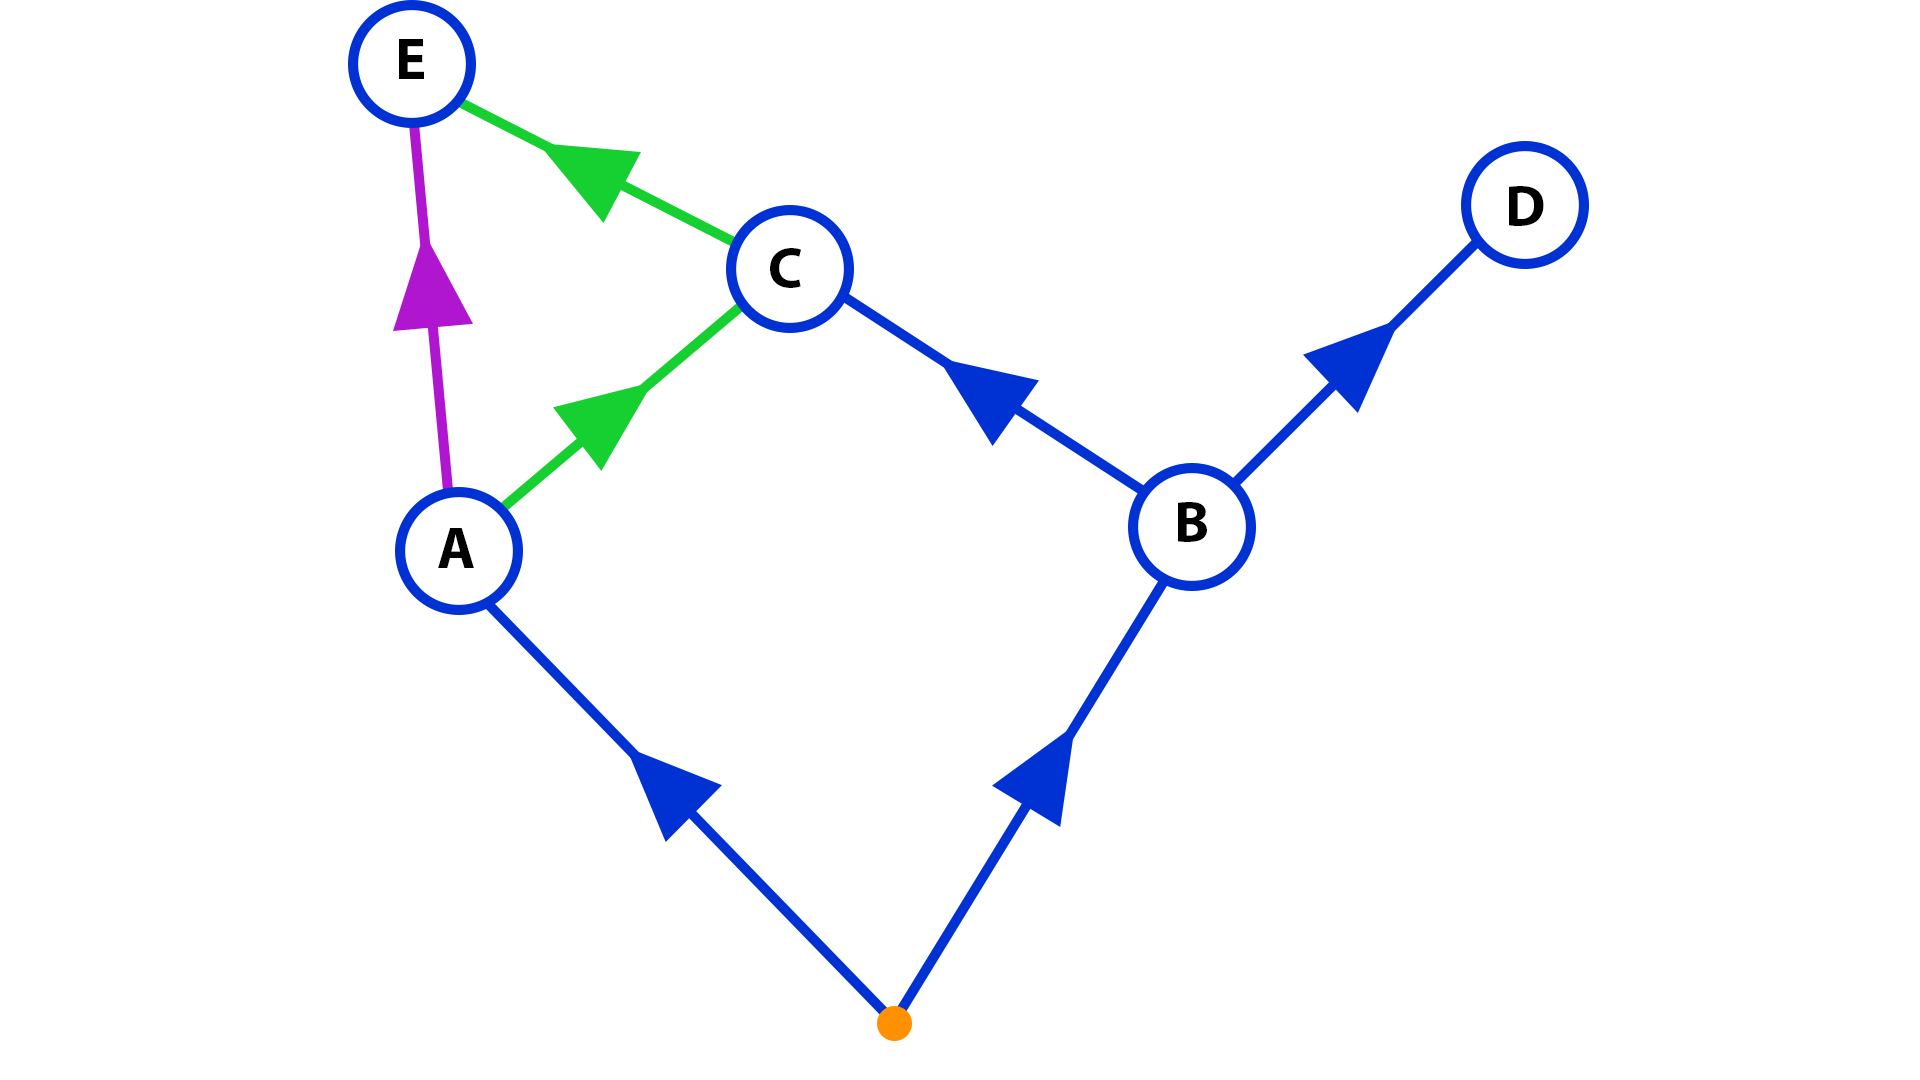
\includegraphics[width=0.7\textwidth,height=\textheight]{../img/Graphs/dfs_A.png}\tabularnewline
Exemple d'un parcours depuis un sommet\tabularnewline
\bottomrule
\end{longtable}

Ici, en partant du sommet A, il y a deux parcours possibles pour arriver
au bout du graphe. En allant jusqu'à E, la distance vaut 1, tandis qu'en
passant pas C pour ensuite arriver au bout, on parcourt une distance de
2. On attribue dans cet exemple une distance de 2 pour le sommet A.
Ainsi, on peut alors dessiner les obstacles dans l'ordre de leur
distance qu'on a évalué précédemment.

\hypertarget{dessins-des-obstacles}{%
\subsection{Dessins des obstacles}\label{dessins-des-obstacles}}

Pour finalement dessiner les obstacles sur la perspective 3D, on prend
chaque obstacle dans l'ordre de la liste créée par le tri de la section
précédente. On utilise les valeurs calculées précédemment \(x_1\),
\(x_2\), \(h_1\) et \(h_2\) qui définissent les coins du polygone final.
La couleur est déterminée par une variable \texttt{this.hex} (valeur
hexadécimale de la couleur) qui est propre à l'obstacle. On utilise une
fonction quadratique qui prend pour abscisse la distance des vecteurs
\texttt{p} et \texttt{h} (vecteurs allant du joueur jusqu'à chacune des
extrémités de l'obstacle) afin de calculer le niveau d'obscurité qu'on
appliquera par un dégradé entre les deux variations de la couleur
initiale. Ceci apporte un air de profondeur, car plus une partie de
l'obstacle est éloignée du joueur, plus celle-ci sera foncée.

\begin{Shaded}
\begin{Highlighting}[]
\KeywordTok{function} \AttributeTok{display3D}\NormalTok{() }\OperatorTok{\{}
    \KeywordTok{const}\NormalTok{ maxl }\OperatorTok{=} \DecValTok{0}\OperatorTok{;}
    \KeywordTok{const}\NormalTok{ minl }\OperatorTok{=} \FloatTok{-0.75}\OperatorTok{;}
    \KeywordTok{const}\NormalTok{ a }\OperatorTok{=} \VariableTok{canvas2D}\NormalTok{.}\AttributeTok{width}\NormalTok{/}\FloatTok{1.2}\OperatorTok{;}
    \KeywordTok{const}\NormalTok{ n }\OperatorTok{=} \DecValTok{2}\OperatorTok{;}

    \KeywordTok{let}\NormalTok{ L1 }\OperatorTok{=} \OperatorTok{-}\NormalTok{((}\KeywordTok{this}\NormalTok{.}\VariableTok{p}\NormalTok{.}\AttributeTok{dist}\NormalTok{ / a) }\OperatorTok{**}\NormalTok{ n)}\OperatorTok{;}
    \ControlFlowTok{if}\NormalTok{ (L1 }\OperatorTok{<}\NormalTok{ minl) L1 }\OperatorTok{=}\NormalTok{ minl}\OperatorTok{;}
    \ControlFlowTok{if}\NormalTok{ (L1 }\OperatorTok{>}\NormalTok{ maxl) L1 }\OperatorTok{=}\NormalTok{ maxl}\OperatorTok{;}

    \KeywordTok{let}\NormalTok{ L2 }\OperatorTok{=} \OperatorTok{-}\NormalTok{((}\KeywordTok{this}\NormalTok{.}\VariableTok{h}\NormalTok{.}\AttributeTok{dist}\NormalTok{ / a) }\OperatorTok{**}\NormalTok{ n)}\OperatorTok{;}
    \ControlFlowTok{if}\NormalTok{ (L2 }\OperatorTok{<}\NormalTok{ minl) L2 }\OperatorTok{=}\NormalTok{ minl}\OperatorTok{;}
    \ControlFlowTok{if}\NormalTok{ (L2 }\OperatorTok{>}\NormalTok{ maxl) L2 }\OperatorTok{=}\NormalTok{ maxl}\OperatorTok{;}

    \KeywordTok{const}\NormalTok{ grd }\OperatorTok{=} \VariableTok{ctx}\NormalTok{.}\AttributeTok{createLinearGradient}\NormalTok{(}
                \KeywordTok{this}\NormalTok{.}\AttributeTok{x1} \OperatorTok{+} \VariableTok{canvas}\NormalTok{.}\AttributeTok{width}\NormalTok{ / }\DecValTok{2}\OperatorTok{,} \VariableTok{canvas}\NormalTok{.}\AttributeTok{height}\NormalTok{ / }\DecValTok{2}\OperatorTok{,}
                \KeywordTok{this}\NormalTok{.}\AttributeTok{x2} \OperatorTok{+} \VariableTok{canvas}\NormalTok{.}\AttributeTok{width}\NormalTok{ / }\DecValTok{2}\OperatorTok{,} \VariableTok{canvas}\NormalTok{.}\AttributeTok{height}\NormalTok{ / }\DecValTok{2}\NormalTok{)}\OperatorTok{;}
    \VariableTok{grd}\NormalTok{.}\AttributeTok{addColorStop}\NormalTok{(}\DecValTok{0}\OperatorTok{,} \AttributeTok{shadeHexColor}\NormalTok{(}\KeywordTok{this}\NormalTok{.}\AttributeTok{hex}\OperatorTok{,}\NormalTok{ L1))}\OperatorTok{;}
    \VariableTok{grd}\NormalTok{.}\AttributeTok{addColorStop}\NormalTok{(}\DecValTok{1}\OperatorTok{,} \AttributeTok{shadeHexColor}\NormalTok{(}\KeywordTok{this}\NormalTok{.}\AttributeTok{hex}\OperatorTok{,}\NormalTok{ L2))}\OperatorTok{;}
    \VariableTok{ctx}\NormalTok{.}\AttributeTok{fillStyle} \OperatorTok{=}\NormalTok{ grd}\OperatorTok{;}

    \AttributeTok{polygon}\NormalTok{([}\KeywordTok{this}\NormalTok{.}\AttributeTok{x1} \OperatorTok{+} \VariableTok{canvas}\NormalTok{.}\AttributeTok{width}\NormalTok{ / }\DecValTok{2}\OperatorTok{,} \KeywordTok{this}\NormalTok{.}\VariableTok{h1}\NormalTok{.}\AttributeTok{h0} \OperatorTok{+} \VariableTok{canvas}\NormalTok{.}\AttributeTok{height}\NormalTok{ / }\DecValTok{2}\OperatorTok{,}
    \KeywordTok{this}\NormalTok{.}\AttributeTok{x1} \OperatorTok{+} \VariableTok{canvas}\NormalTok{.}\AttributeTok{width}\NormalTok{ / }\DecValTok{2}\OperatorTok{,} \KeywordTok{this}\NormalTok{.}\VariableTok{h1}\NormalTok{.}\AttributeTok{h1} \OperatorTok{+} \VariableTok{canvas}\NormalTok{.}\AttributeTok{height}\NormalTok{ /}\DecValTok{2}\OperatorTok{,}
    \KeywordTok{this}\NormalTok{.}\AttributeTok{x2} \OperatorTok{+} \VariableTok{canvas}\NormalTok{.}\AttributeTok{width}\NormalTok{ / }\DecValTok{2}\OperatorTok{,} \KeywordTok{this}\NormalTok{.}\VariableTok{h2}\NormalTok{.}\AttributeTok{h1} \OperatorTok{+} \VariableTok{canvas}\NormalTok{.}\AttributeTok{height}\NormalTok{ /}\DecValTok{2}\OperatorTok{,}
    \KeywordTok{this}\NormalTok{.}\AttributeTok{x2} \OperatorTok{+} \VariableTok{canvas}\NormalTok{.}\AttributeTok{width}\NormalTok{ / }\DecValTok{2}\OperatorTok{,} \KeywordTok{this}\NormalTok{.}\VariableTok{h2}\NormalTok{.}\AttributeTok{h0} \OperatorTok{+} \VariableTok{canvas}\NormalTok{.}\AttributeTok{height}\NormalTok{ /}\DecValTok{2}
\NormalTok{    ]}\OperatorTok{,} \VerbatimStringTok{`grd`}\OperatorTok{,} \DecValTok{2}\NormalTok{)}\OperatorTok{;}
\OperatorTok{\}}
\end{Highlighting}
\end{Shaded}

\hypertarget{conclusion}{%
\section{Conclusion}\label{conclusion}}

Pour récapituler, l'implémentation de ma nouvelle méthode pour un moteur
de rendu 3D avec le Raycasting a été réussie. Je suis parti de l'idée de
créer un moteur de jeu à partir de la méthode utilisée dans les premiers
jeux vidéos 3D comme \emph{Wolfenstein 3D} ou \emph{Doom}. Après avoir
été insatisfait de l'aspect du rendu 3D, j'ai poussé les limites qui
auraient été infranchissables avec les capacités de calculs des
ordinateurs de l'époque et j'ai pu moderniser la technique en gardant la
simplicité du concept. J'ai créé une nouvelle méthode qui s'inspire
d'une idée simple de l'ancienne, mais qui exploite pleinement les
capacités des appareils d'aujourd'hui.

À travers la réalisation du projet, j'ai appris à appliquer des notions
de géométrie vectorielle qu'on m'enseignait à l'école en parallèle. J'ai
également étudié la théorie des graphes pour comprendre les algorithmes
de triage et les POSETs. Grâce à ce projet, j'ai appris à confronter des
problèmes sortant du cadre de mes connaissances et chercher des
solutions de manière autonome.

La création de l'interface graphique est également un élément de la
version finale dont je suis très fier. Je n'avais pas beaucoup
d'expérience dans ce domaine et j'ai appris des techniques qui me seront
extrêmement utiles pour mes projets à venir. J'ai dû comprendre comment
créer une interface dynamique qui est assurée d'être adaptée à la taille
de l'écran ainsi que la possibilité d'accéder aux mêmes fonctionnalités
à la fois sur ordinateur et sur écran tactile.

La version finale de mon projet ressemble exactement à ce que
j'imaginais pouvoir créer lorsque j'ai commencé à travailler dessus il y
a un an et demi. Par ce fait, je prends une grande satisfaction à
pouvoir montrer mon site web depuis mon téléphone à mes amis et à ma
famille.

Après avoir passé plusieurs centaines d'heures à travailler sur ce
projet, je suis extrêmement fier du résultat et je me réjouis de pouvoir
l'utiliser comme tremplin pour explorer des nouvelles techniques de
programmation. Les leçons que j'en ai tirées au cours de sa réalisation
me sont très utiles pour l'avenir. Maintenant, on peut réellement se
plonger dans ce monde qui semble être un espace 3D, mais qui ne l'est
pas vraiment.

\hypertarget{annexe}{%
\section{Annexe}\label{annexe}}

\hypertarget{a-trouver-lintersection-de-deux-segments}{%
\subsection{a) Trouver l'intersection de deux
segments}\label{a-trouver-lintersection-de-deux-segments}}

Soit Px, Py, les coordonnées du point d'intersection des deux segments
définis par (\(x_1\) , \(y_1\) ) et (\(x_2\) , \(y_2\) ) pour le premier
et (\(x_3\) , \(y_3\) ) et (\(x_4\) , \(y_4\) ) pour le deuxième. Ainsi,
on pose \(t\), \(u\) tel que :

\[
t = \frac{(x_1 − x_3)(𝑦_3 − 𝑦_4) − (𝑦_1 − 𝑦_3) (x_3 − x_4)}
         {(x_1 − x_2) ∗ (y_3 − y_4) − (y_1 − y_2) ∗ (x_3 − x_4)}
    \mathrm{\quad et \quad}
u = \frac{(x_1 − x_3) (y_1 − y_2) − (y_1 − y_3) (x_1 − x_2)}
         {(x_1 − x_2) ∗ (y_3 − y_4) − (y_1 − y_2) ∗ (x_3 − x_4)}
\]

On note que le dénominateur est le même pour le calcul de \(u\) et de
\(t\).

Ces deux formules sont le résultat d'un développement d'un calcul de
déterminants\footnote{Line-line intersection. Wikipédia : l'encyclopédie
  libre {[}en ligne{]}. Dernière modification de la page le 6 octobre
  2021 à 21:04. {[}Consulté le 9 octobre 2021{]}. Disponible à
  l'adresse:
  \url{https://en.wikipedia.org/wiki/Line\%E2\%80\%93line_intersection}}
(notion associée aux matrices).

Avant même de calculer le point \(P_x\) et \(P_y\), là où se trouve
l'intersection des deux segments, on peut vérifier si cette intersection
existe.

L'intersection des deux segments existe si \(0.0 \leq t \geq 1.0\) et
\(0.0 \leq u \geq 1.0\). Ceci permet d'ignorer le résultat et de
seulement savoir s'il y a une intersection afin d'optimiser le
programme.

En revanche, on peut quand même calculer \(P_x\) et \(P_y\) tels que :

\[
(P_x, P_y) = (x_3 + u(x_4 - x_3), y_3 + u(y_4 - y_3))
\]

Dans mon code, j'ai deux fonctions en lien avec l'intersection :
\emph{Intersection()} qui détermine les coordonnées d'un point
d'intersection de deux segments s'il existe, et \emph{isIntersection()}
qui fait de même sans calculer les coordonnées.

\begin{Shaded}
\begin{Highlighting}[]
\KeywordTok{function} \AttributeTok{isIntersection}\NormalTok{(w1}\OperatorTok{,}\NormalTok{ w2) }\OperatorTok{\{}
    \KeywordTok{const}\NormalTok{ x1 }\OperatorTok{=} \VariableTok{w1}\NormalTok{.}\VariableTok{pos}\NormalTok{.}\AttributeTok{x}\OperatorTok{;}
    \KeywordTok{const}\NormalTok{ y1 }\OperatorTok{=} \VariableTok{w1}\NormalTok{.}\VariableTok{pos}\NormalTok{.}\AttributeTok{y}\OperatorTok{;}
    \KeywordTok{const}\NormalTok{ x2 }\OperatorTok{=}\NormalTok{ x1 }\OperatorTok{+} \VariableTok{w1}\NormalTok{.}\VariableTok{dir}\NormalTok{.}\AttributeTok{x} \OperatorTok{*} \VariableTok{w1}\NormalTok{.}\VariableTok{dir}\NormalTok{.}\AttributeTok{length}\OperatorTok{;}
    \KeywordTok{const}\NormalTok{ y2 }\OperatorTok{=}\NormalTok{ y1 }\OperatorTok{+} \VariableTok{w1}\NormalTok{.}\VariableTok{dir}\NormalTok{.}\AttributeTok{y} \OperatorTok{*} \VariableTok{w1}\NormalTok{.}\VariableTok{dir}\NormalTok{.}\AttributeTok{length}\OperatorTok{;}
    \KeywordTok{const}\NormalTok{ x3 }\OperatorTok{=} \VariableTok{w2}\NormalTok{.}\VariableTok{pos}\NormalTok{.}\AttributeTok{x}\OperatorTok{;}
    \KeywordTok{const}\NormalTok{ y3 }\OperatorTok{=} \VariableTok{w2}\NormalTok{.}\VariableTok{pos}\NormalTok{.}\AttributeTok{y}\OperatorTok{;}
    \KeywordTok{const}\NormalTok{ x4 }\OperatorTok{=}\NormalTok{ x3 }\OperatorTok{+} \VariableTok{w2}\NormalTok{.}\VariableTok{dir}\NormalTok{.}\AttributeTok{x}\OperatorTok{;}
    \KeywordTok{const}\NormalTok{ y4 }\OperatorTok{=}\NormalTok{ y3 }\OperatorTok{+} \VariableTok{w2}\NormalTok{.}\VariableTok{dir}\NormalTok{.}\AttributeTok{y}\OperatorTok{;}
    \KeywordTok{const}\NormalTok{ den }\OperatorTok{=}\NormalTok{ (x1 }\OperatorTok{-}\NormalTok{ x2) }\OperatorTok{*}\NormalTok{ (y3 }\OperatorTok{-}\NormalTok{ y4) }\OperatorTok{-}\NormalTok{ (y1 }\OperatorTok{-}\NormalTok{ y2) }\OperatorTok{*}\NormalTok{ (x3 }\OperatorTok{-}\NormalTok{ x4)}\OperatorTok{;}
    \ControlFlowTok{if}\NormalTok{ (den }\OperatorTok{==} \DecValTok{0}\NormalTok{) }\ControlFlowTok{return} \KeywordTok{false}\OperatorTok{;}
\CommentTok{// Si le dénominateur est égal à 0, le calcul engendrerait une erreur}
\CommentTok{// donc l'intersection n'existe forcément pas}
    \KeywordTok{const}\NormalTok{ t }\OperatorTok{=}\NormalTok{ ((x1 }\OperatorTok{-}\NormalTok{ x3) }\OperatorTok{*}\NormalTok{ (y3 }\OperatorTok{-}\NormalTok{ y4) }\OperatorTok{-}\NormalTok{ (y1 }\OperatorTok{-}\NormalTok{ y3) }\OperatorTok{*}\NormalTok{ (x3 }\OperatorTok{-}\NormalTok{ x4)) / den}\OperatorTok{;}
    \KeywordTok{const}\NormalTok{ u }\OperatorTok{=} \OperatorTok{-}\NormalTok{((x1 }\OperatorTok{-}\NormalTok{ x2) }\OperatorTok{*}\NormalTok{ (y1 }\OperatorTok{-}\NormalTok{ y3) }\OperatorTok{-}\NormalTok{ (y1 }\OperatorTok{-}\NormalTok{ y2) }\OperatorTok{*}\NormalTok{ (x1 }\OperatorTok{-}\NormalTok{ x3)) / den}\OperatorTok{;}

\CommentTok{// Si l’intersection existe, on retourne vrai ou faux.}
    \ControlFlowTok{return}\NormalTok{ u }\OperatorTok{>=} \DecValTok{0} \OperatorTok{&&}\NormalTok{ u }\OperatorTok{<=} \DecValTok{1} \OperatorTok{&&}\NormalTok{ t }\OperatorTok{>=} \DecValTok{0} \OperatorTok{&&}\NormalTok{ t }\OperatorTok{<=} \DecValTok{1}\OperatorTok{;}
\OperatorTok{\}}

\KeywordTok{function} \AttributeTok{intersection}\NormalTok{(w1}\OperatorTok{,}\NormalTok{ w2) }\OperatorTok{\{}
\CommentTok{// On n’effectuera aucun calcul si aucune intersection n’existe!}
    \ControlFlowTok{if}\NormalTok{ (}\OperatorTok{!}\AttributeTok{isIntersection}\NormalTok{(w1}\OperatorTok{,}\NormalTok{ w2)) }\ControlFlowTok{return}\OperatorTok{;}

    \KeywordTok{const}\NormalTok{ x1 }\OperatorTok{=} \VariableTok{w1}\NormalTok{.}\VariableTok{pos}\NormalTok{.}\AttributeTok{x}\OperatorTok{;}
    \KeywordTok{const}\NormalTok{ y1 }\OperatorTok{=} \VariableTok{w1}\NormalTok{.}\VariableTok{pos}\NormalTok{.}\AttributeTok{y}\OperatorTok{;}
    \KeywordTok{const}\NormalTok{ x2 }\OperatorTok{=}\NormalTok{ x1 }\OperatorTok{+} \VariableTok{w1}\NormalTok{.}\VariableTok{dir}\NormalTok{.}\AttributeTok{x} \OperatorTok{*} \VariableTok{w1}\NormalTok{.}\VariableTok{dir}\NormalTok{.}\AttributeTok{length}\OperatorTok{;}
    \KeywordTok{const}\NormalTok{ y2 }\OperatorTok{=}\NormalTok{ y1 }\OperatorTok{+} \VariableTok{w1}\NormalTok{.}\VariableTok{dir}\NormalTok{.}\AttributeTok{y} \OperatorTok{*} \VariableTok{w1}\NormalTok{.}\VariableTok{dir}\NormalTok{.}\AttributeTok{length}\OperatorTok{;}
    \KeywordTok{const}\NormalTok{ x3 }\OperatorTok{=} \VariableTok{w2}\NormalTok{.}\VariableTok{pos}\NormalTok{.}\AttributeTok{x}\OperatorTok{;}
    \KeywordTok{const}\NormalTok{ y3 }\OperatorTok{=} \VariableTok{w2}\NormalTok{.}\VariableTok{pos}\NormalTok{.}\AttributeTok{y}\OperatorTok{;}
    \KeywordTok{const}\NormalTok{ x4 }\OperatorTok{=}\NormalTok{ x3 }\OperatorTok{+} \VariableTok{w2}\NormalTok{.}\VariableTok{dir}\NormalTok{.}\AttributeTok{x}\OperatorTok{;}
    \KeywordTok{const}\NormalTok{ y4 }\OperatorTok{=}\NormalTok{ y3 }\OperatorTok{+} \VariableTok{w2}\NormalTok{.}\VariableTok{dir}\NormalTok{.}\AttributeTok{y}\OperatorTok{;}

    \KeywordTok{const}\NormalTok{ den }\OperatorTok{=}\NormalTok{ (x1 }\OperatorTok{-}\NormalTok{ x2) }\OperatorTok{*}\NormalTok{ (y3 }\OperatorTok{-}\NormalTok{ y4) }\OperatorTok{-}\NormalTok{ (y1 }\OperatorTok{-}\NormalTok{ y2) }\OperatorTok{*}\NormalTok{ (x3 }\OperatorTok{-}\NormalTok{ x4)}\OperatorTok{;}
    \KeywordTok{const}\NormalTok{ u }\OperatorTok{=}\NormalTok{ ((x2 }\OperatorTok{-}\NormalTok{ x1) }\OperatorTok{*}\NormalTok{ (y1 }\OperatorTok{-}\NormalTok{ y3) }\OperatorTok{-}\NormalTok{ (y2 }\OperatorTok{-}\NormalTok{ y1) }\OperatorTok{*}\NormalTok{ (x1 }\OperatorTok{-}\NormalTok{ x3)) / den}\OperatorTok{;}

    \KeywordTok{const}\NormalTok{ xint }\OperatorTok{=}\NormalTok{ x3 }\OperatorTok{+}\NormalTok{ u }\OperatorTok{*}\NormalTok{ (x4 }\OperatorTok{-}\NormalTok{ x3)}\OperatorTok{;}
    \KeywordTok{const}\NormalTok{ yint }\OperatorTok{=}\NormalTok{ y3 }\OperatorTok{+}\NormalTok{ u }\OperatorTok{*}\NormalTok{ (y4 }\OperatorTok{-}\NormalTok{ y3)}\OperatorTok{;}
    \KeywordTok{const}\NormalTok{ intersection }\OperatorTok{=} \OperatorTok{\{}
        \StringTok{'x'}\OperatorTok{:}\NormalTok{ xint}\OperatorTok{,}
        \StringTok{'y'}\OperatorTok{:}\NormalTok{ yint}\OperatorTok{,}
            \CommentTok{// Formule pour calculer la distance entre deux points}
        \StringTok{'dist'}\OperatorTok{:} \VariableTok{Math}\NormalTok{.}\AttributeTok{sqrt}\NormalTok{((y1 }\OperatorTok{-}\NormalTok{ yint) }\OperatorTok{**} \DecValTok{2} \OperatorTok{+}\NormalTok{ (x1 }\OperatorTok{-}\NormalTok{ xint) }\OperatorTok{**} \DecValTok{2}\NormalTok{)}
    \OperatorTok{\};}
    \ControlFlowTok{return}\NormalTok{ intersection}\OperatorTok{;}
\OperatorTok{\}}
\end{Highlighting}
\end{Shaded}

\hypertarget{b-trouver-si-deux-vecteurs-sont-orientuxe9s-dans-le-sens-des-aiguilles-dune-montre}{%
\subsection{b) Trouver si deux vecteurs sont orientés dans le sens des
aiguilles d'une
montre}\label{b-trouver-si-deux-vecteurs-sont-orientuxe9s-dans-le-sens-des-aiguilles-dune-montre}}

Une fonction beaucoup utilisée dans mon programme s'appelle
\emph{isClockwiseOrder()}. Cette fonction retourne vrai si le premier
vecteur inséré est orienté de telle sorte qu'il vient avant le deuxième
dans le sens des aiguilles d'une montre. Ceci me permet de comparer
l'orientation de deux vecteurs sans me soucier de leur angle relatif.
L'opération qui se trouve derrière cette fonction est le produit
vectoriel.

Comme nous sommes sur un plan en 2D on appliquera le produit vectoriel
\(a \times b \text{ avec } a_z = 0 \text{ et } b_z = 0\):

\[
a \times b =
\begin{pmatrix}
a_x \\
a_y \\
0
\end{pmatrix}
\times
\begin{pmatrix}
b_x \\
b_y \\
0
\end{pmatrix} =
\begin{pmatrix}
a_y \cdot \color{red}{0} - \color{red}{0} \cdot b_y \\
\color{red}{0} \cdot b_x - a_x \cdot \color{red}{0} \\
a_x \cdot b_y - a_y \cdot b_x
\end{pmatrix} =
\begin{pmatrix}
0 \\
0 \\
a_x \cdot b_y - a_y \cdot b_x
\end{pmatrix}
\]

Ceci simplifie les calculs à effectuer et réduit le résultat à une
valeur seulement. Cette valeur représente un certain vecteur
perpendiculaire au plan 2D dont la hauteur est déterminée par le calcul.
Ainsi, par la règle d'anticommutativité du produit vectoriel,
(c'est-a-dire que \(a \times b = −b \times a\)), on peut facilement
déterminer si deux vecteurs sont orientés dans le sens des aiguilles
d'une montre.

\begin{longtable}[]{@{}c@{}}
\toprule
\endhead
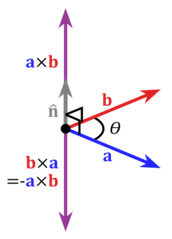
\includegraphics[width=\textwidth,height=0.25\textheight]{../img/Drawings/anticommutativite.png}\tabularnewline
L'anticommutativité du produit vectoriel\footnote{Représentation de
  l'anticommutativité du produit vectoriel, (auteur inconnu), 2008,
  Disponible à l'adresse:
  \url{https://commons.wikimedia.org/wiki/File:Cross_product_vector.svg}}\tabularnewline
\bottomrule
\end{longtable}

En conclusion, si le résultat de \(a_x \cdot b_x − a_y \cdot b_x\) est
positif, alors \(a\) et \(b\) sont orientés dans le sens des aiguilles
d'une montre. S'il est négatif, alors \(a\) et \(b\) sont orientés dans
le sens contraire des aiguilles d'une montre. S'il est égal à 0, alors
les vecteurs sont parallèles. Dans mon code, je considère que ce cas est
équivalent au premier par simplification.

\begin{Shaded}
\begin{Highlighting}[]
\KeywordTok{function} \AttributeTok{isClockwiseOrder}\NormalTok{(v1}\OperatorTok{,}\NormalTok{ v2) }\OperatorTok{\{}
    \ControlFlowTok{return} \VariableTok{v1}\NormalTok{.}\AttributeTok{x}\OperatorTok{*}\VariableTok{v2}\NormalTok{.}\AttributeTok{y} \OperatorTok{-} \VariableTok{v1}\NormalTok{.}\AttributeTok{y}\OperatorTok{*}\VariableTok{v2}\NormalTok{.}\AttributeTok{x} \OperatorTok{<=} \DecValTok{0}\OperatorTok{;}
\OperatorTok{\}}
\end{Highlighting}
\end{Shaded}

\hypertarget{bibliographie}{%
\section{Bibliographie}\label{bibliographie}}

\hypertarget{images}{%
\subsection{Images}\label{images}}

\begin{itemize}
\item
  Page de titre : Vue d'obstacles multicolores en perspective ; Image
  générée à partir de mon code, HAMELINK Marcus 2021
\item
  The cross product with respect to a right-handed coordinate system
  (auteur inconnu), 2008, Disponible à l'adresse~:
  \url{https://en.wikipedia.org/wiki/Cross_product\#/media/File:Cross_product_vector.svg}
\item
  Représentation schématique des valeurs ; Schéma que j'ai dessiné,
  HAMELINK Marcus 2021
\item
  Schémas pour illustrer la comparaison entre deux obstacles ; Schémas
  que j'ai dessinés, HAMELINK Marcus 2021
\end{itemize}

\hypertarget{sources}{%
\subsection{Sources}\label{sources}}

\begin{itemize}
\item
  Raycasting. Wikipédia : l'encyclopédie libre {[}en ligne{]}. Dernière
  modification de la page le 22 juillet 2021 à 22:17. {[}Consulté le 10
  octobre 2021{]}. Disponible à l'adresse :
  \url{https://fr.wikipedia.org/wiki/Raycasting}
\item
  SHIFFMAN Daniel, 2019. Coding Challenge \#146 : Rendering Raycasting
  {[}enregistrement vidéo{]}. Youtube {[}en ligne{]}. Disponible à
  l'adresse : \url{https://youtu.be/vYgIKn7iDH8}
\item
  Line-line intersection. Wikipédia : l'encyclopédie libre {[}en
  ligne{]}. Dernière modification de la page le 6 octobre 2021 à 21:04.
  {[}Consulté le 14 octobre 2021{]}. Disponible à l'adresse :
  \url{https://en.wikipedia.org/wiki/Line\%E2\%80\%93line_intersection}
\item
  VANDEVENNE Lode, 2004-2021. Lode's Computer Graphics Tutorial :
  Raycasting {[}en ligne{]}. Dernière modification de la page en 2020.
  {[}Consulté le 15 janvier 2021{]} Lode Vandevenne, 2004-2020.
  Disponible à l'adresse :
  \url{https://lodev.org/cgtutor/raycasting.html}
\end{itemize}

\end{document}
